\chapter{实验与讨论}
本章对前面提到的所有模型设计了相应的实验,同时做了多组对照试验,以验证模型改进的可行性和有效性。

\section{实验数据集与预处理}
\subsection{实验数据集}
实验开始前调研了与本文任务类似的数据集,调研结果发现高质量的可用于跨界服务平台的中文语料数据集相对匮乏,例如对话类数据集部分输入为语音而不是
文本,再如科大讯飞阿里小蜜有着海量有商业价值数据的公司没有公开数据集。为此,我们选择在已有数据集上做标注补充和扩展,构建了跨界服务相关的中文
预料数据集。

\begin{figure}[htbp]
    \centering
    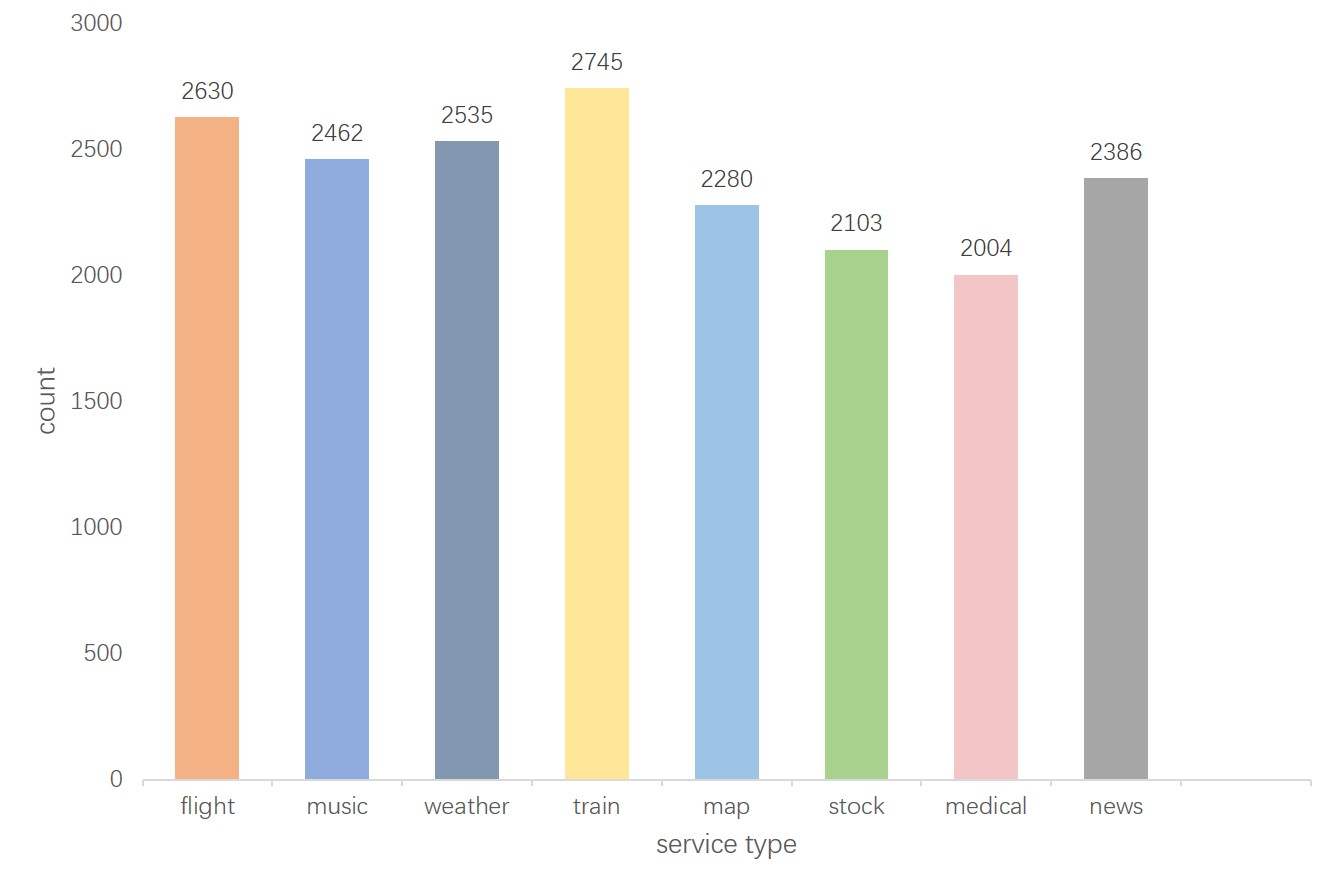
\includegraphics[width=15cm]{./images/count.jpg}
    \caption{数据集分布图}
    \label{fig:count}
  \end{figure}

SMP2019中文人机对话技术评测自然语言理解任务中提供了SMP2019ECDT数据集,其中主要包括垂直类,闲聊类和知识问答,我们结合跨界服务平台系统内部常用
服务,从垂直类中选择部分数据做标注扩充以及数据扩充。本文筛选了跨界服务平台中用户使用较多的几类服务的语料信息,包括“航班flight”,“音乐music”,
“天气weather”,“火车train”,“地图map”,“股票stock”,“医疗medical”,“新闻news”共八大类服务,再根据这些服务的接口构建接口类别的全集,例如“query”,“play”,“order”等;同时确定了服务接口以后,服务接口调用
时的参数(语义槽)也就确定了,例如“songName”,“singer”,“startCity”,“endCity”等,可见接口和服务参数都是和服务强相关的。例如,当服务类型被判定为
“天气weather”时,接口类型为“query”,参数(语义槽)为“city”。

SMP2019ECDT数据集中与跨界服务平台系统内八大服务相关的数据量并不大,因此本文对原有数据集做了扩充。扩充工作主要分为两部分:横向扩充和纵向扩充,横向
扩充的直觉来源于同一个语义的句子不同人的表述会不同,例如“杭州具体天气怎么样?”和“杭州今天多少度?”,因此考虑对同种语义的句子做横向扩充,这里我们借助
了百度和必应(微软bing)两大搜索引擎的搜索联想补全功能。横向扩充完的句子标签中的服务类别和接口类别不用变,只需要修改语义槽标注。
如图\ref{fig:baidu},\ref{fig:bing}所示,想要扩展火车服务的查询接口的语料数据,再搜索引擎输入“成都到杭州火车”,利用搜索引擎的联想补全功能
达到扩充的目的。

\begin{figure}[htbp]
    \centering
    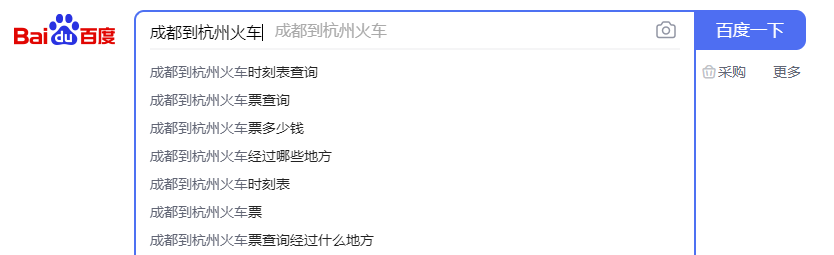
\includegraphics[width=15cm]{./images/baidu.png}
    \caption{数据横向扩充图1}
    \label{fig:baidu}
  \end{figure}

  \begin{figure}[htbp]
    \centering
    
\includegraphics[width=15cm]{./images/bing.png}
    \caption{数据横向扩充图2}
    \label{fig:bing}
  \end{figure}

数据集纵向扩充是组织跨界服务课题组和实验室同学填写问卷,让被调研者输入相应服务的查询语句,收集起来对语句进行人工标注,完成数据集的扩容。
每个人对同一语义的表达会有差异,有差异的数据对训练出泛化能力好的数据是大有裨益的。最终经过课题组同学的努力,共构建了19145条数据组成实验
数据集,每条数据都包含服务类别标签、接口类别标签和参数(语义槽)标签。

\subsection{预处理}

\section{评价指标}
评价指标用于评估模型的性能,对于服务分类任务,本文采用准确率(Accuracy)来评估模型;对于接口分类
任务,同样采用准确率(Accuracy)来评估模型;对于参数(语义槽)填充任务,采用$F_1$值来评估模型。同时引入
句子准确率(Sentence Accuracy)作为更严格的指标来评估模型,即一个句子只有在三项任务同时正确时才会被计入
句子准确率中。

 \begin{table}[htb]
      \centering
      \caption{服务类型混淆矩阵}
      \label{tab:hunxiao}
  \begin{tabular}{c|c|c|c|c|c|c|c|c|c}
    \toprule
    \multicolumn{2}{c|}{\multirow{2}{*}{}}&
    \multicolumn{8}{c}{预测值}\\
    \cline{3-10}
    \multicolumn{2}{c|}{}&flight & music & weather & train & map &stock &medical & news \\
     \hline
     \multirow{8}{*}{真实值}&
     flight&$n_1$&$n_2$&$n_3$&$n_4$&$n_5$&$n_6$&$n_7$&$n_8$\\
     \cline{2-10}
     \multicolumn{1}{c|}{}&music&$n_{9}$&$n_{10}$&$n_{11}$&$n_{12}$&$n_{13}$&$n_{14}$&$n_{15}$&$n_{16}$\\
     \cline{2-10}
     \multicolumn{1}{c|}{}&weather&$n_{17}$&$n_{18}$&$n_{19}$&$n_{20}$&$n_{21}$&$n_{22}$&$n_{23}$&$n_{24}$\\
     \cline{2-10}
     \multicolumn{1}{c|}{}&train&$n_{25}$&$n_{26}$&$n_{27}$&$n_{28}$&$n_{29}$&$n_{30}$&$n_{31}$&$n_{32}$\\
     \cline{2-10}
     \multicolumn{1}{c|}{}&map&$n_{33}$&$n_{34}$&$n_{35}$&$n_{36}$&$n_{37}$&$n_{38}$&$n_{39}$&$n_{40}$\\
     \cline{2-10}
     \multicolumn{1}{c|}{}&stock&$n_{41}$&$n_{42}$&$n_{43}$&$n_{44}$&$n_{45}$&$n_{46}$&$n_{47}$&$n_{48}$\\
     \cline{2-10}
     \multicolumn{1}{c|}{}&medical&$n_{49}$&$n_{50}$&$n_{51}$&$n_{52}$&$n_{53}$&$n_{54}$&$n_{55}$&$n_{56}$\\
     \cline{2-10}
     \multicolumn{1}{c|}{}&news&$n_{57}$&$n_{58}$&$n_{59}$&$n_{60}$&$n_{61}$&$n_{62}$&$n_{63}$&$n_{64}$\\
    \bottomrule
    \end{tabular}
  \end{table}

  以服务类别标签的混淆矩阵\ref{tab:hunxiao}为例介绍以上指标的计算方法,设样本数据总量是N。
  准确率(Accuracy)是最直观的性能指标,它是正确预测的观测值与总观测值的比率,如果具有很高的准确率,可以认为模型是很好的:
  \begin{equation}
  % \text {Accuracy}(\text {health})=\frac{\sum_{i=8}^{14} n_{i}}{N}
  \text {Accuracy}=\frac{n_1+n_{10}+n_{19}+n_{28}+n_{37}+n_{46}+n_{55}+n_{64}}{N}
\end{equation}
精确度(Precision)是正确预测的该类样本与总的预测为该类样本的观察值之比,多用于二分类问题,对于文本分类这样的多分类问题,可以单独取一个类别做计算,以天气类别为例:
\begin{equation}
  \text {Precision}(\text {weather})=\frac{n_{19}}{n_3+n_{11}+n_{19}+n_{27}+n_{35}+n_{43}+n_{51}+n_{69}}
\end{equation}
召回率(Recall)是正确预测的该类样本与实际为该类的样本总量的比率,多用于二分类问题,对于文本分类这样的多分类问题,可以单独取一个类别做计算,以天气类别为例:
\begin{equation}
  \text {Recall}(\text {weather})=\frac{n_{19}}{\sum_{i=17}^{24} n_{i}}
\end{equation}
F1值是精确度和召回率的调和平均值,直观上它不如准确性容易理解,但是F1通常比准确性更有用,尤其是在类分布不均匀的情况下:
\begin{equation}
  F_1=\frac{2 \times Precision \times Recall}{ Precision + Recall}
  % F_{1}=\frac{2 \times \text {Precision } \times \text { Recall}}{\text {Precision }+\text { Recall}}
\end{equation}

\section{实验设置}
\subsection{实验环境}
本文的实验环境是实验室服务器,操作系统为Ubuntu 16.04.4系统,集成开发环境选用Pycharm使用Python语言利用PyTorch框架编程。
关于实验室机器硬件配置,中央处理器为Intel(R) Xeon(R) CPU E5-2603 v3 @ 1.60GHz,图形处理器为GeForce RTX 2080Ti。

\begin{table}[htb]
  \centering
  \caption{实验环境}
  \label{tab:hunxiao}
\begin{tabular}{c|c}
\hline
实验环境&配置参数\\
\hline
操作系统&Ubuntu 16.04.4\\
编程语言&python 3.6\\
IDE&Pycharm\\
模型框架&PyTorch\\
\hline
\end{tabular}
\end{table}

\subsection{超参数设置}
超参数的调整主要利用验证集依靠控制变量法来寻找最优的超参数值,同一实验进行多次训练取最优。例如,卷积层的激活函数本文对比了ReLu、Tanh、PReLU,
CNN层卷积核高度对比了2,3,4三种,卷积核的数量进行了16,32,64,128四种不同的实验等,比较不同超参数对实验结果的影响。
attention-CNN-LSTM模型和Transformable-CNN-LSTM模型中CNN层最终确定的超参数值如表\ref{tab:cnnPara}所示,
引入预训练的模型最终确定的超参数值如表\ref{tab:bertPara}所示,

\begin{table}[htb]
  \centering
  \caption{CNN层相关参数选择}
  \label{tab:cnnPara}
\begin{tabular}{cc|cc}
\hline
参数名称&值&参数名称&值\\
\hline
卷积核高度&2,3&卷积核数量&64\\
learning rate&0.002&batch size&128\\
池化层方法&k-max polling&epochs &60\\
Optimizer&Adam&&\\
\hline
\end{tabular}
\end{table}

\begin{table}[htb]
  \centering
  \caption{引入预训练的模型相关参数选择}
  \label{tab:bertPara}
\begin{tabular}{cc|cc}
\hline
参数名称&值&参数名称&值\\
\hline
learning rate&5e-4&batch size&64\\
Optimizer&Adam&epochs &20\\
堆叠层数N&2&&\\
\hline
\end{tabular}
\end{table}

\section{实验设计}
本文对前两章提到的所有模型都进行了实验,虽然模型数量较多,但总的来说可分为两类:基于词向量的模型和引入预训练的模型
\subsection{基于词向量的模型}
前文提到的attention-CNN-LSTM模型、Transformable-CNN-LSTM模型、BiLSTM-attention-CRF模型均是基于词向量的模型,实验流程类似。
第一步输入句子经过分词处理得到词序列,接着利用word2vec将词语向量化输入神经网络训练。训练集数据用于模型的拟合,验证集数据用于对模型超参数的调整以及对模型性能做初步判定,
测试集用来评估模型最终的泛化能力,不作为调参、特征等算法相关的选择依据。测试阶段加载训练好的模型参数,数据输入进入网络得到预测结果。
\begin{figure}[htbp]
  \centering
  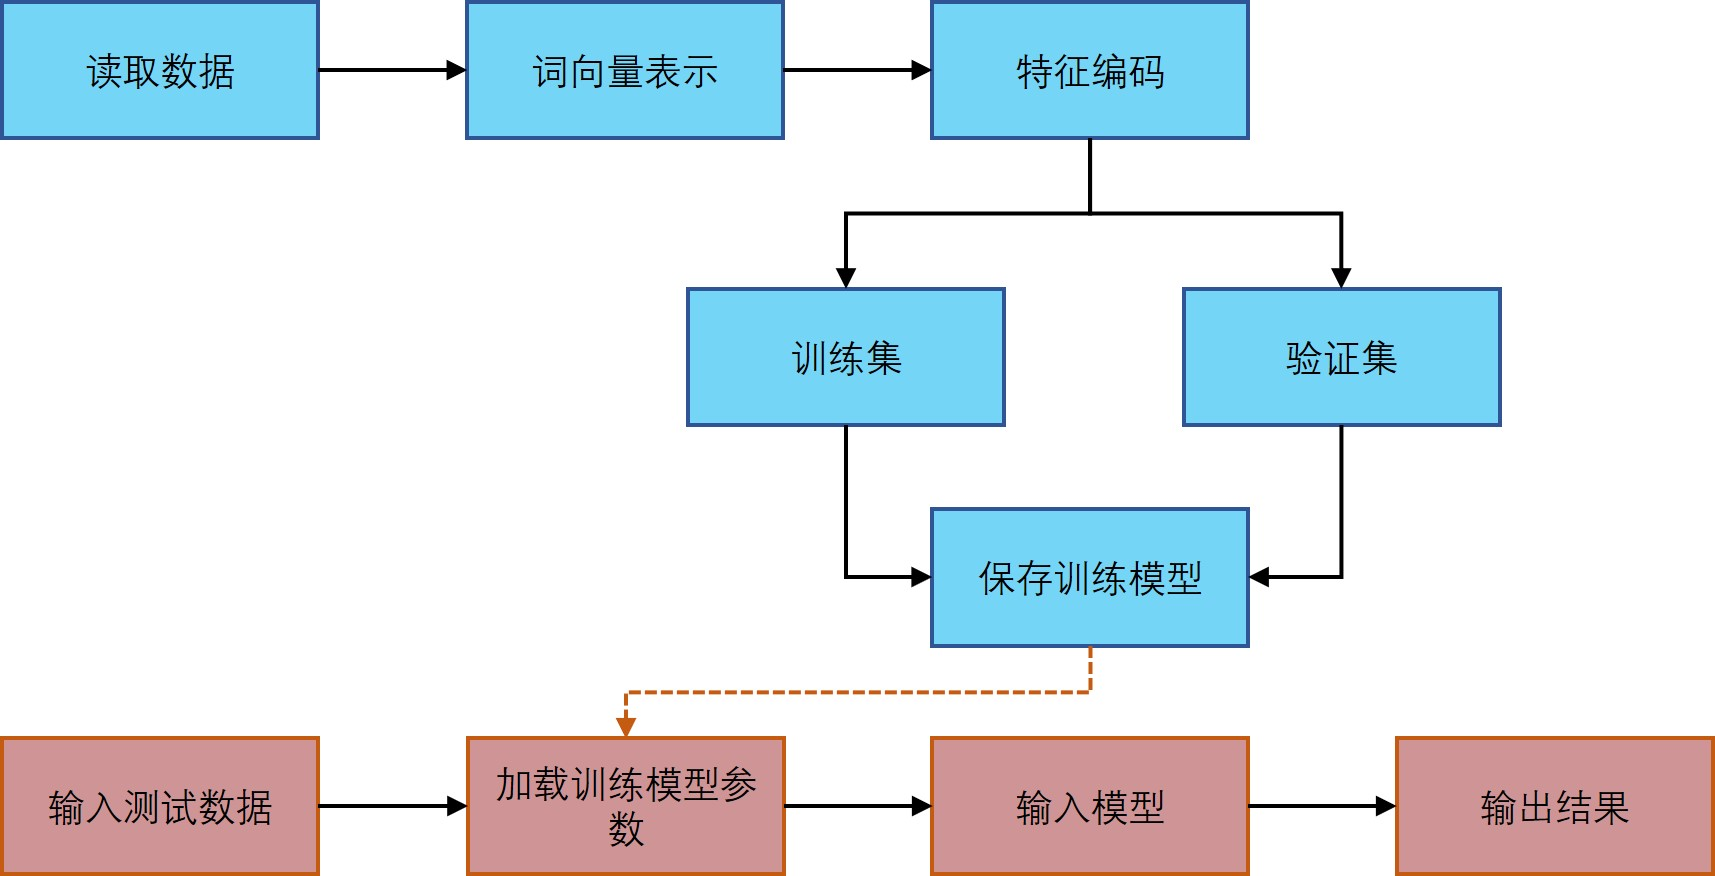
\includegraphics[scale=0.4]{./images/word2vecTrain.jpg}
  \caption{基于词向量模型的实验流程}
  \label{fig:word2vecTrain}
\end{figure}

\subsection{引入预训练的模型}
前文提到的单向联合识别模型、交互式联合识别模型、bert-base联合识别模型、引入bert的交互式联合识别模型均属于结合预训练的模型,实验流程类似。
首先加载预训练模型的参数,输入句子的字序列向量进入网络训练。训练集数据用于模型的拟合以及对预训练模型进行微调(fine-tuning),验证集数据用于对模型超参数的调整以及对模型性能做初步判定,
测试集用来评估模型最终的泛化能力,不作为调参、特征等算法相关的选择依据。测试阶段加载训练好的模型参数和预训练参数,数据输入进入网络得到预测结果。
\begin{figure}[htbp]
  \centering
  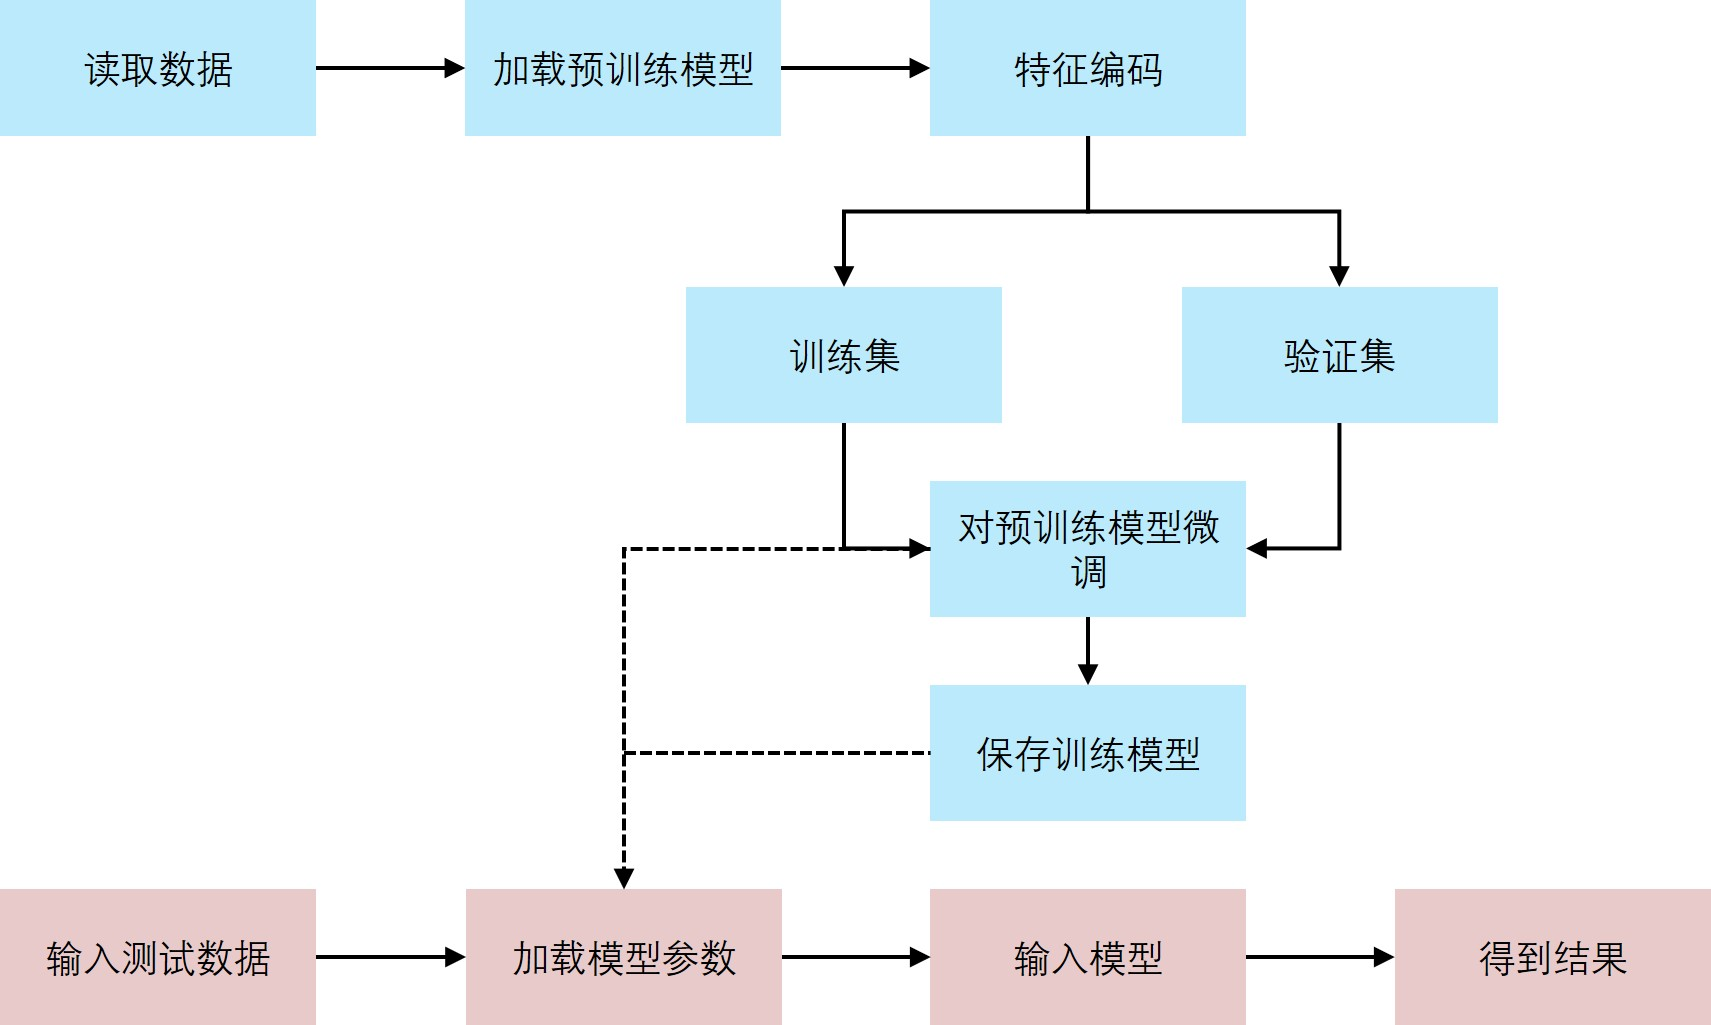
\includegraphics[scale=0.4]{./images/bertTrain.jpg}
  \caption{引入预训练模型的实验流程}
  \label{fig:bertTrain}
\end{figure}


\section{实验结果与分析}

\begin{figure}[htbp]
  % \centering
  % \hspace{-7mm}
  \subfloat[ATT-CLSTM loss值变化曲线]{
  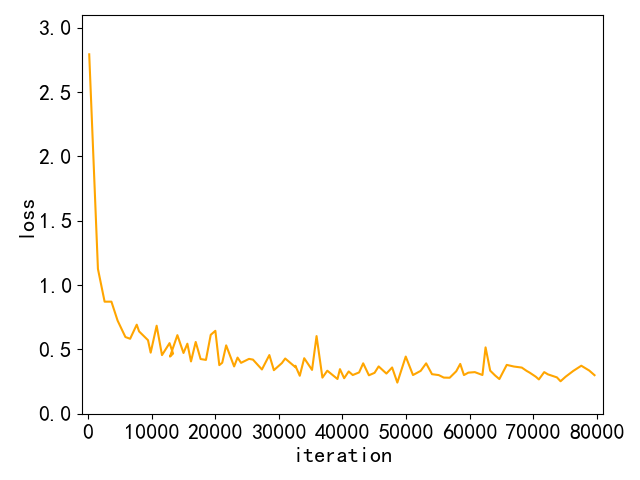
\includegraphics[width=8cm]{./images/bad.png}
  \label{fig:88888}
  }
  % \hspace{5pt}
    % \hspace{+5mm}
  \subfloat[BERT-base loss值变化曲线]{
  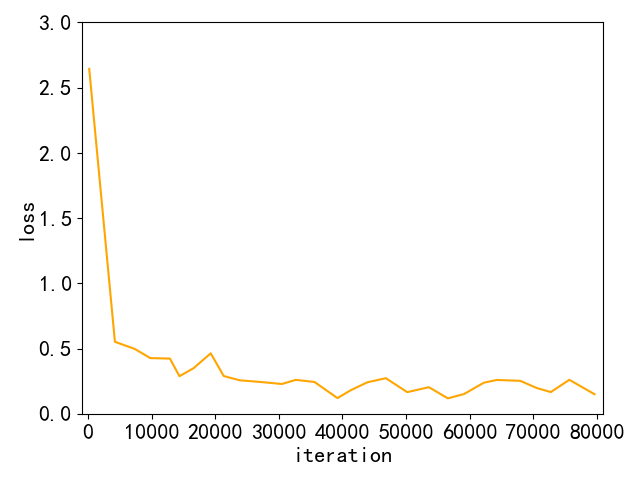
\includegraphics[width=8cm]{./images/good.png}
  \label{fig:88}
  }
  \caption{训练集loss值变化曲线}
  \label{fig:loss}
  \end{figure}

本实验模型众多且多数模型loss曲线走势相近,我们从结果中选择两类
有代表性的曲线走势展开分析,分别是基于词向量模型的ATT-CLSTM和基于bert的BERT-base,他们的损失函数Loss曲线变化如图\ref{fig:loss}所示,
可以看到经过多轮迭代后模型得到充分训练并趋于收敛,但结合了预训练模型的BERT-base相比于词向量的模型loss在收敛时震荡更小,收敛更快,最终结果也更优。

\begin{figure}[htbp]
  % \centering
  % \hspace{-7mm}
  \subfloat[服务Service分类的accuracy曲线]{
  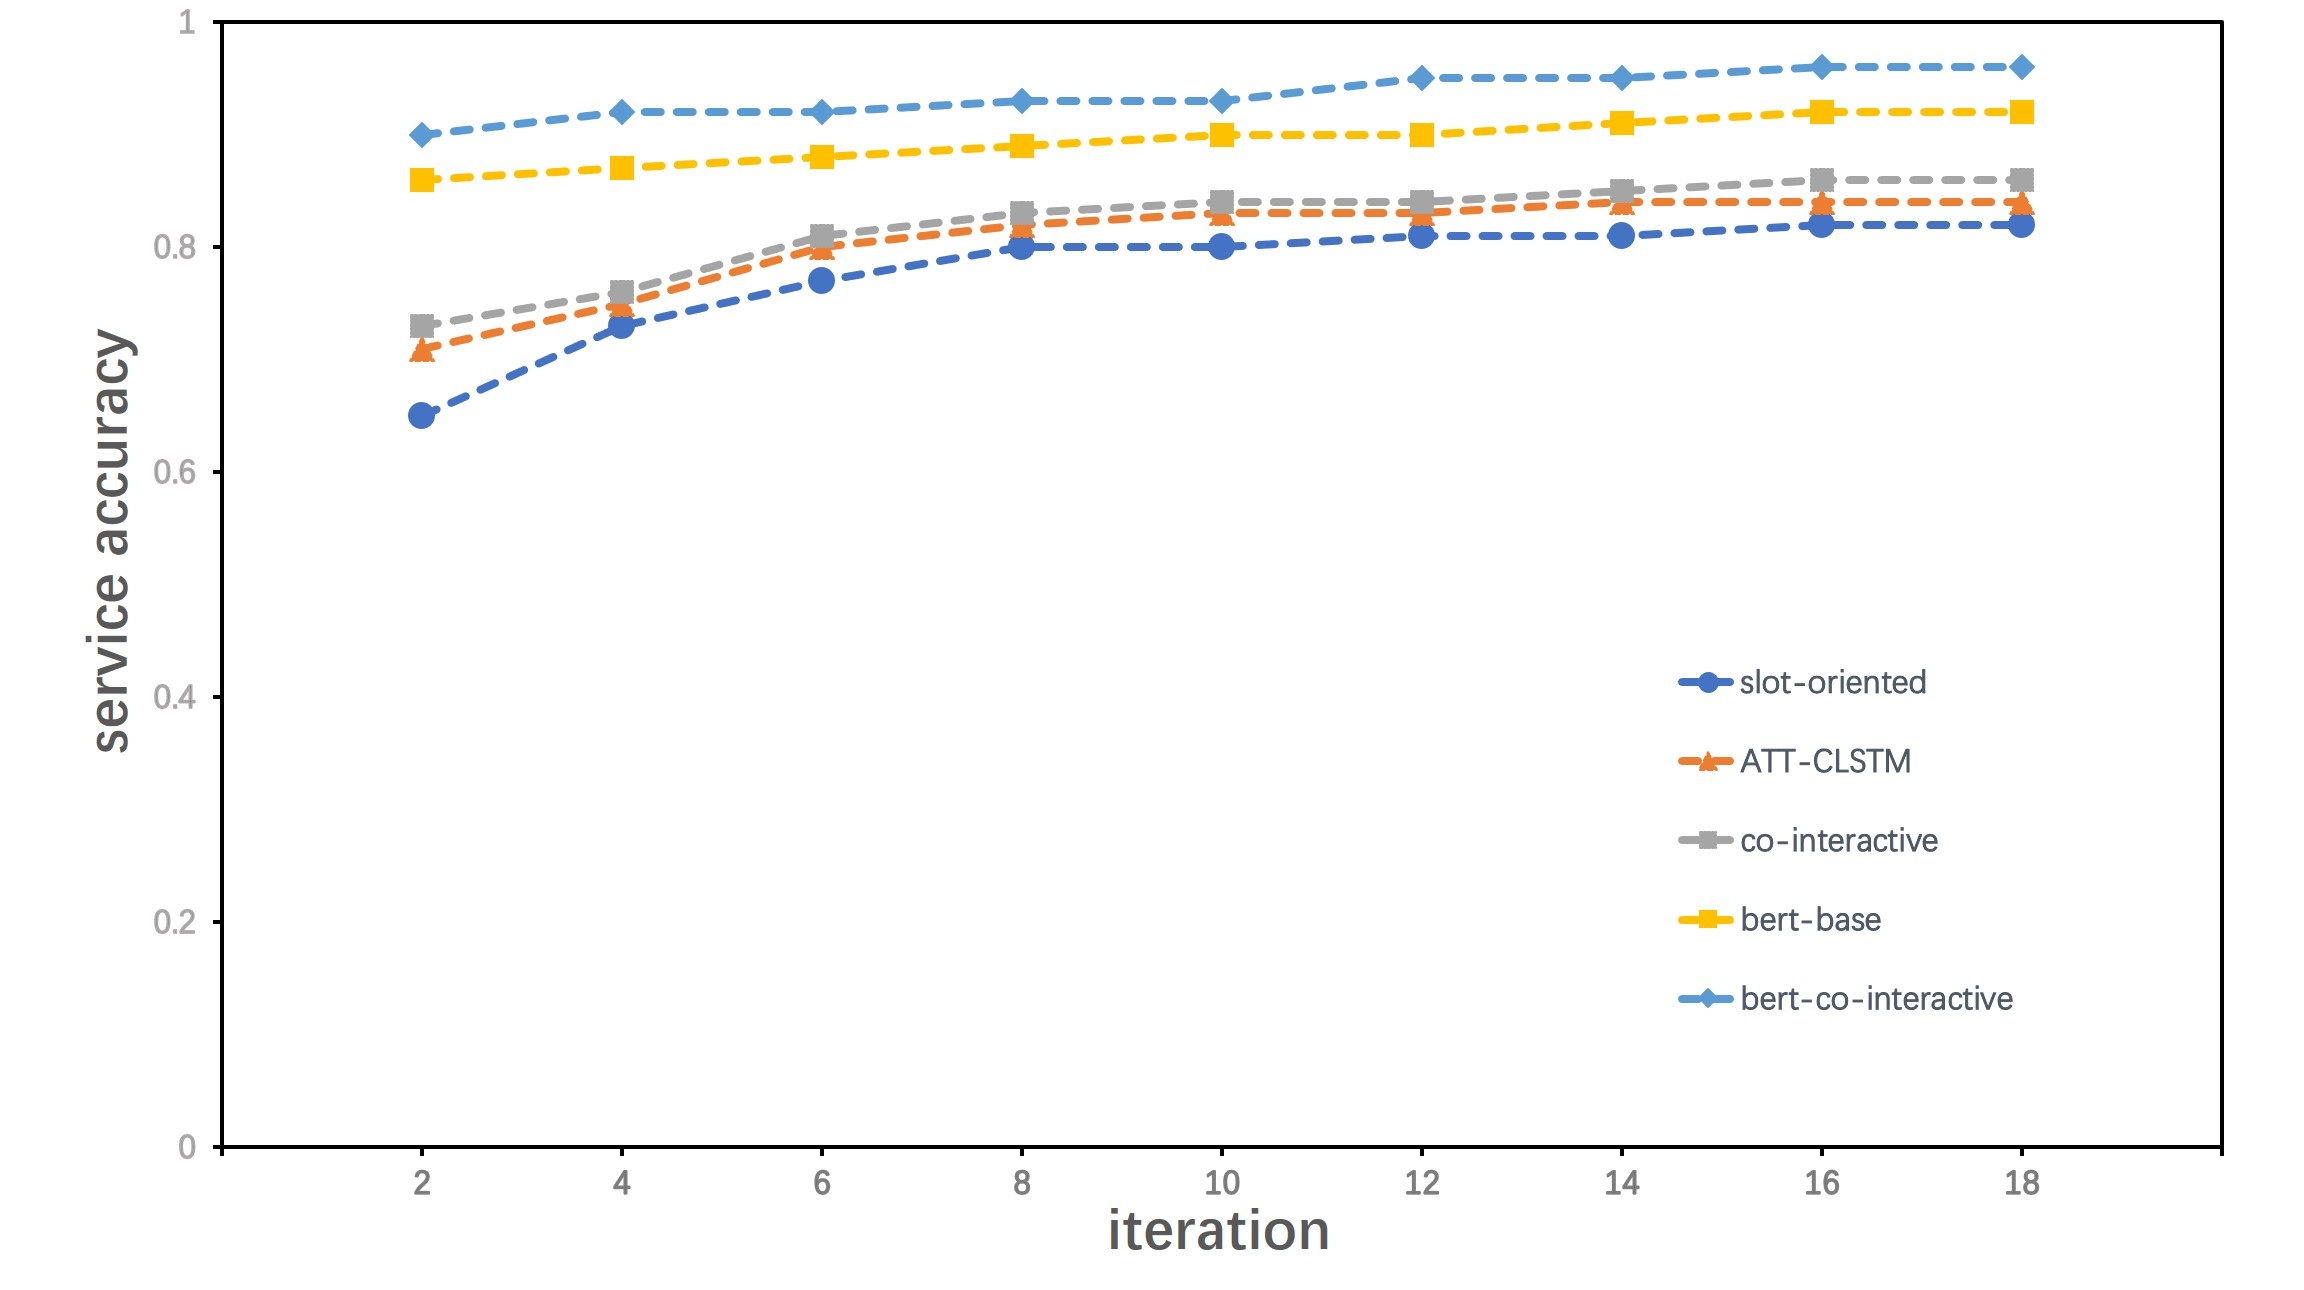
\includegraphics[width=8.6cm]{./images/serviceAccuracy.jpg}
  \label{fig:serviceAccuracy}
  }
  % \hspace{5pt}
    % \hspace{+5mm}
  \subfloat[接口Interface分类的accuracy曲线]{
  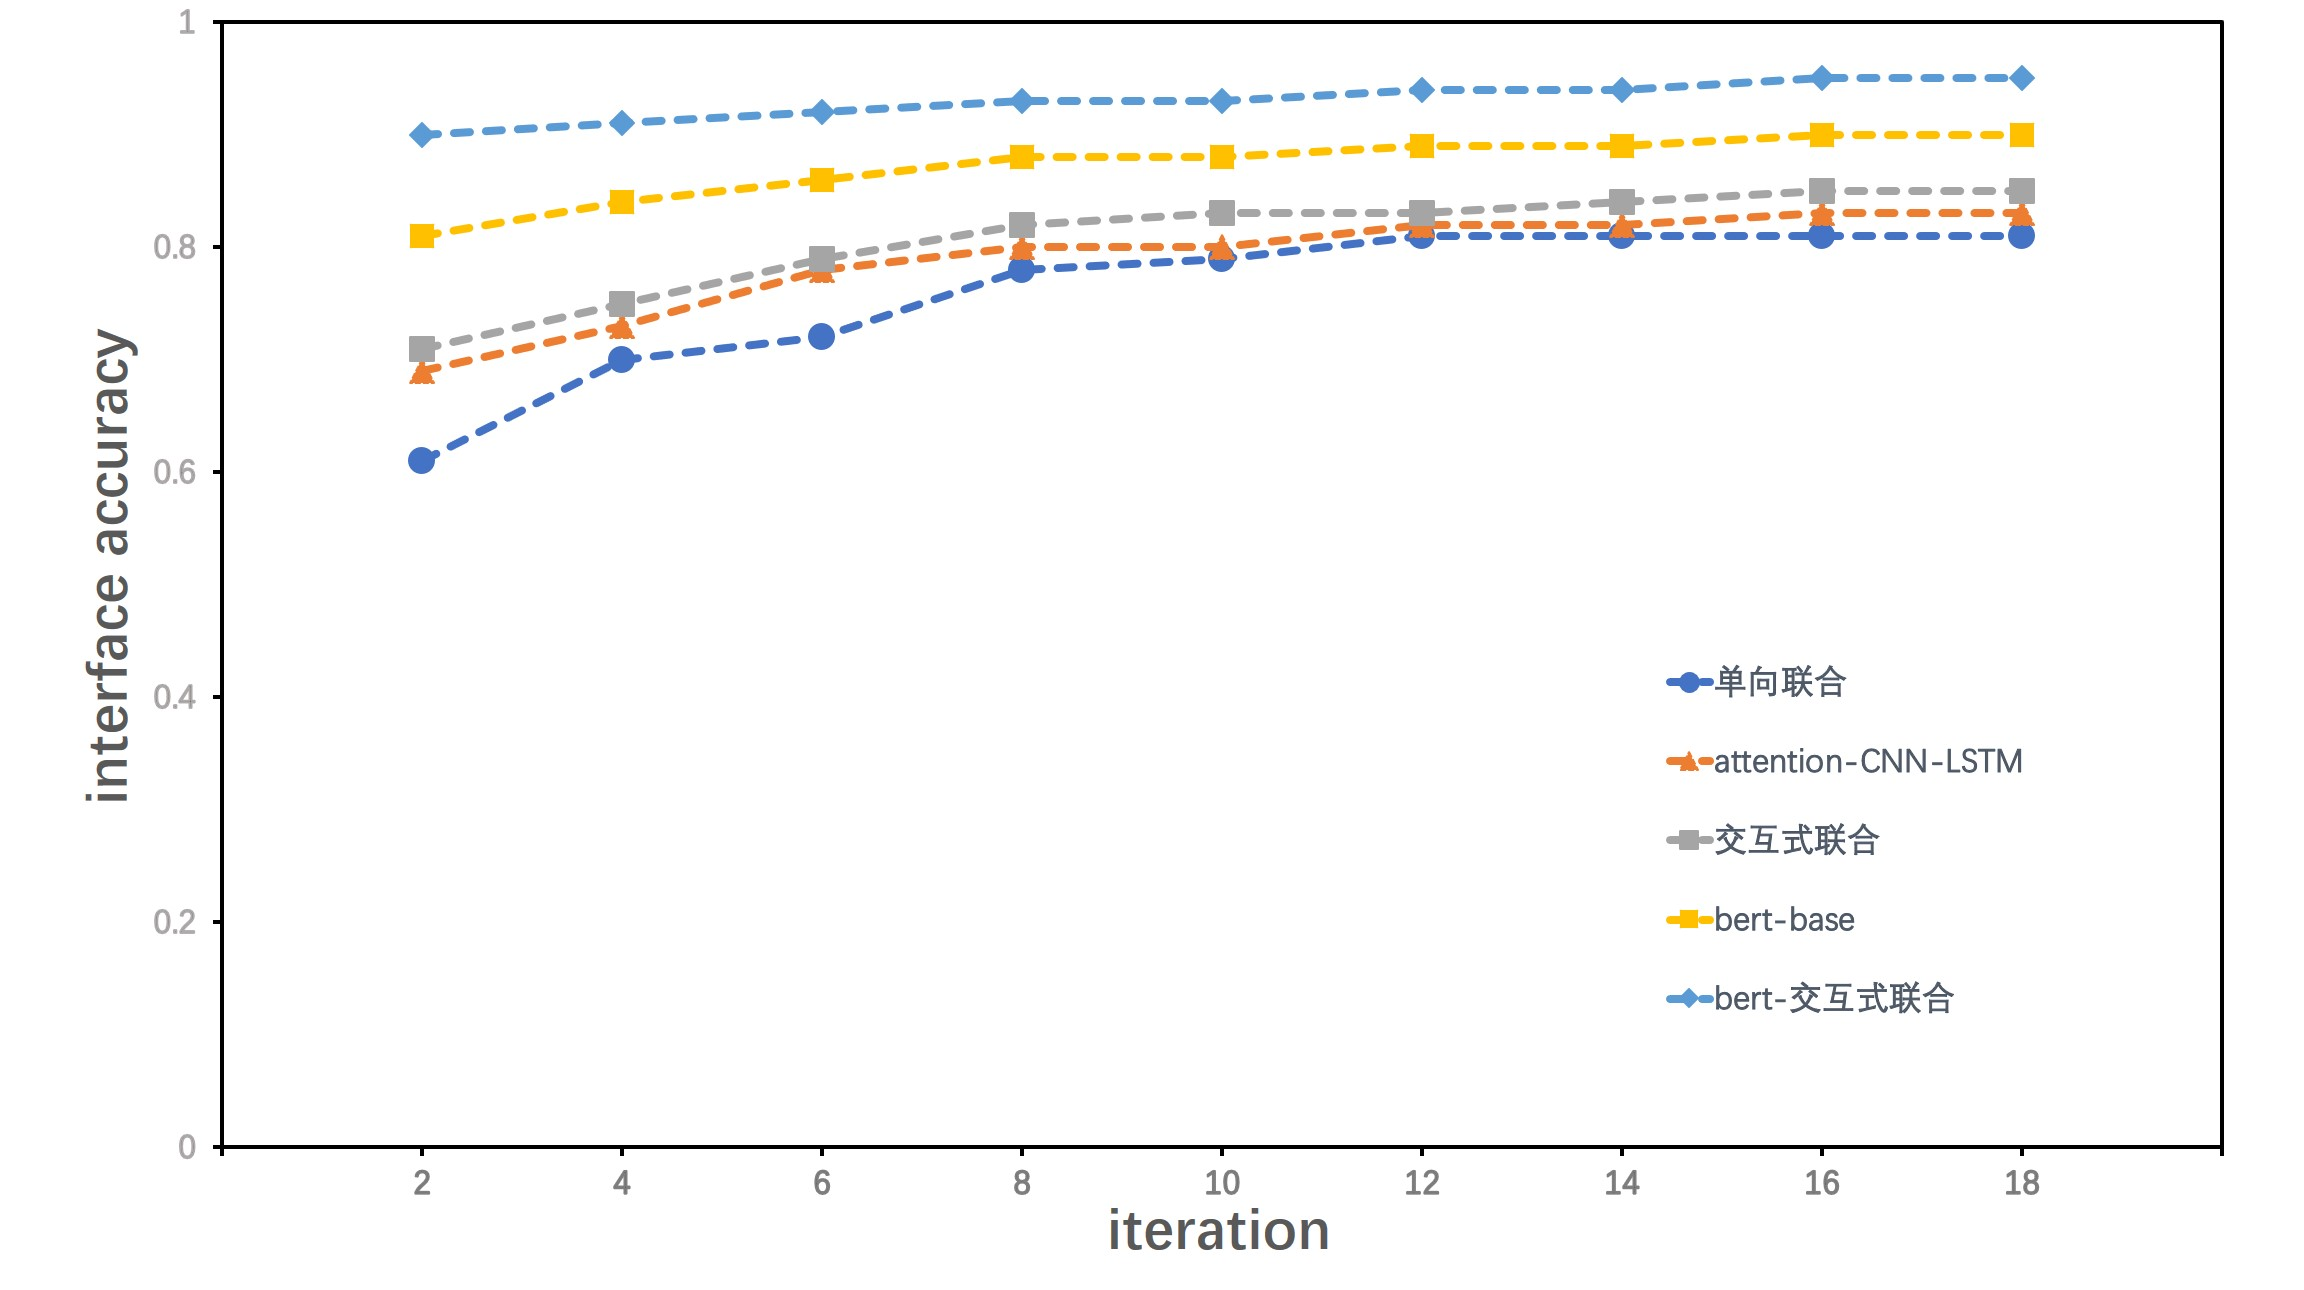
\includegraphics[width=8.6cm]{./images/interfaceAccuracy.jpg}
  \label{fig:interfaceAccuracy}
  }\\
  % \hspace{5pt}
  %  \hspace{-7mm}
  \subfloat[语义槽填充的$F_1$曲线]{
  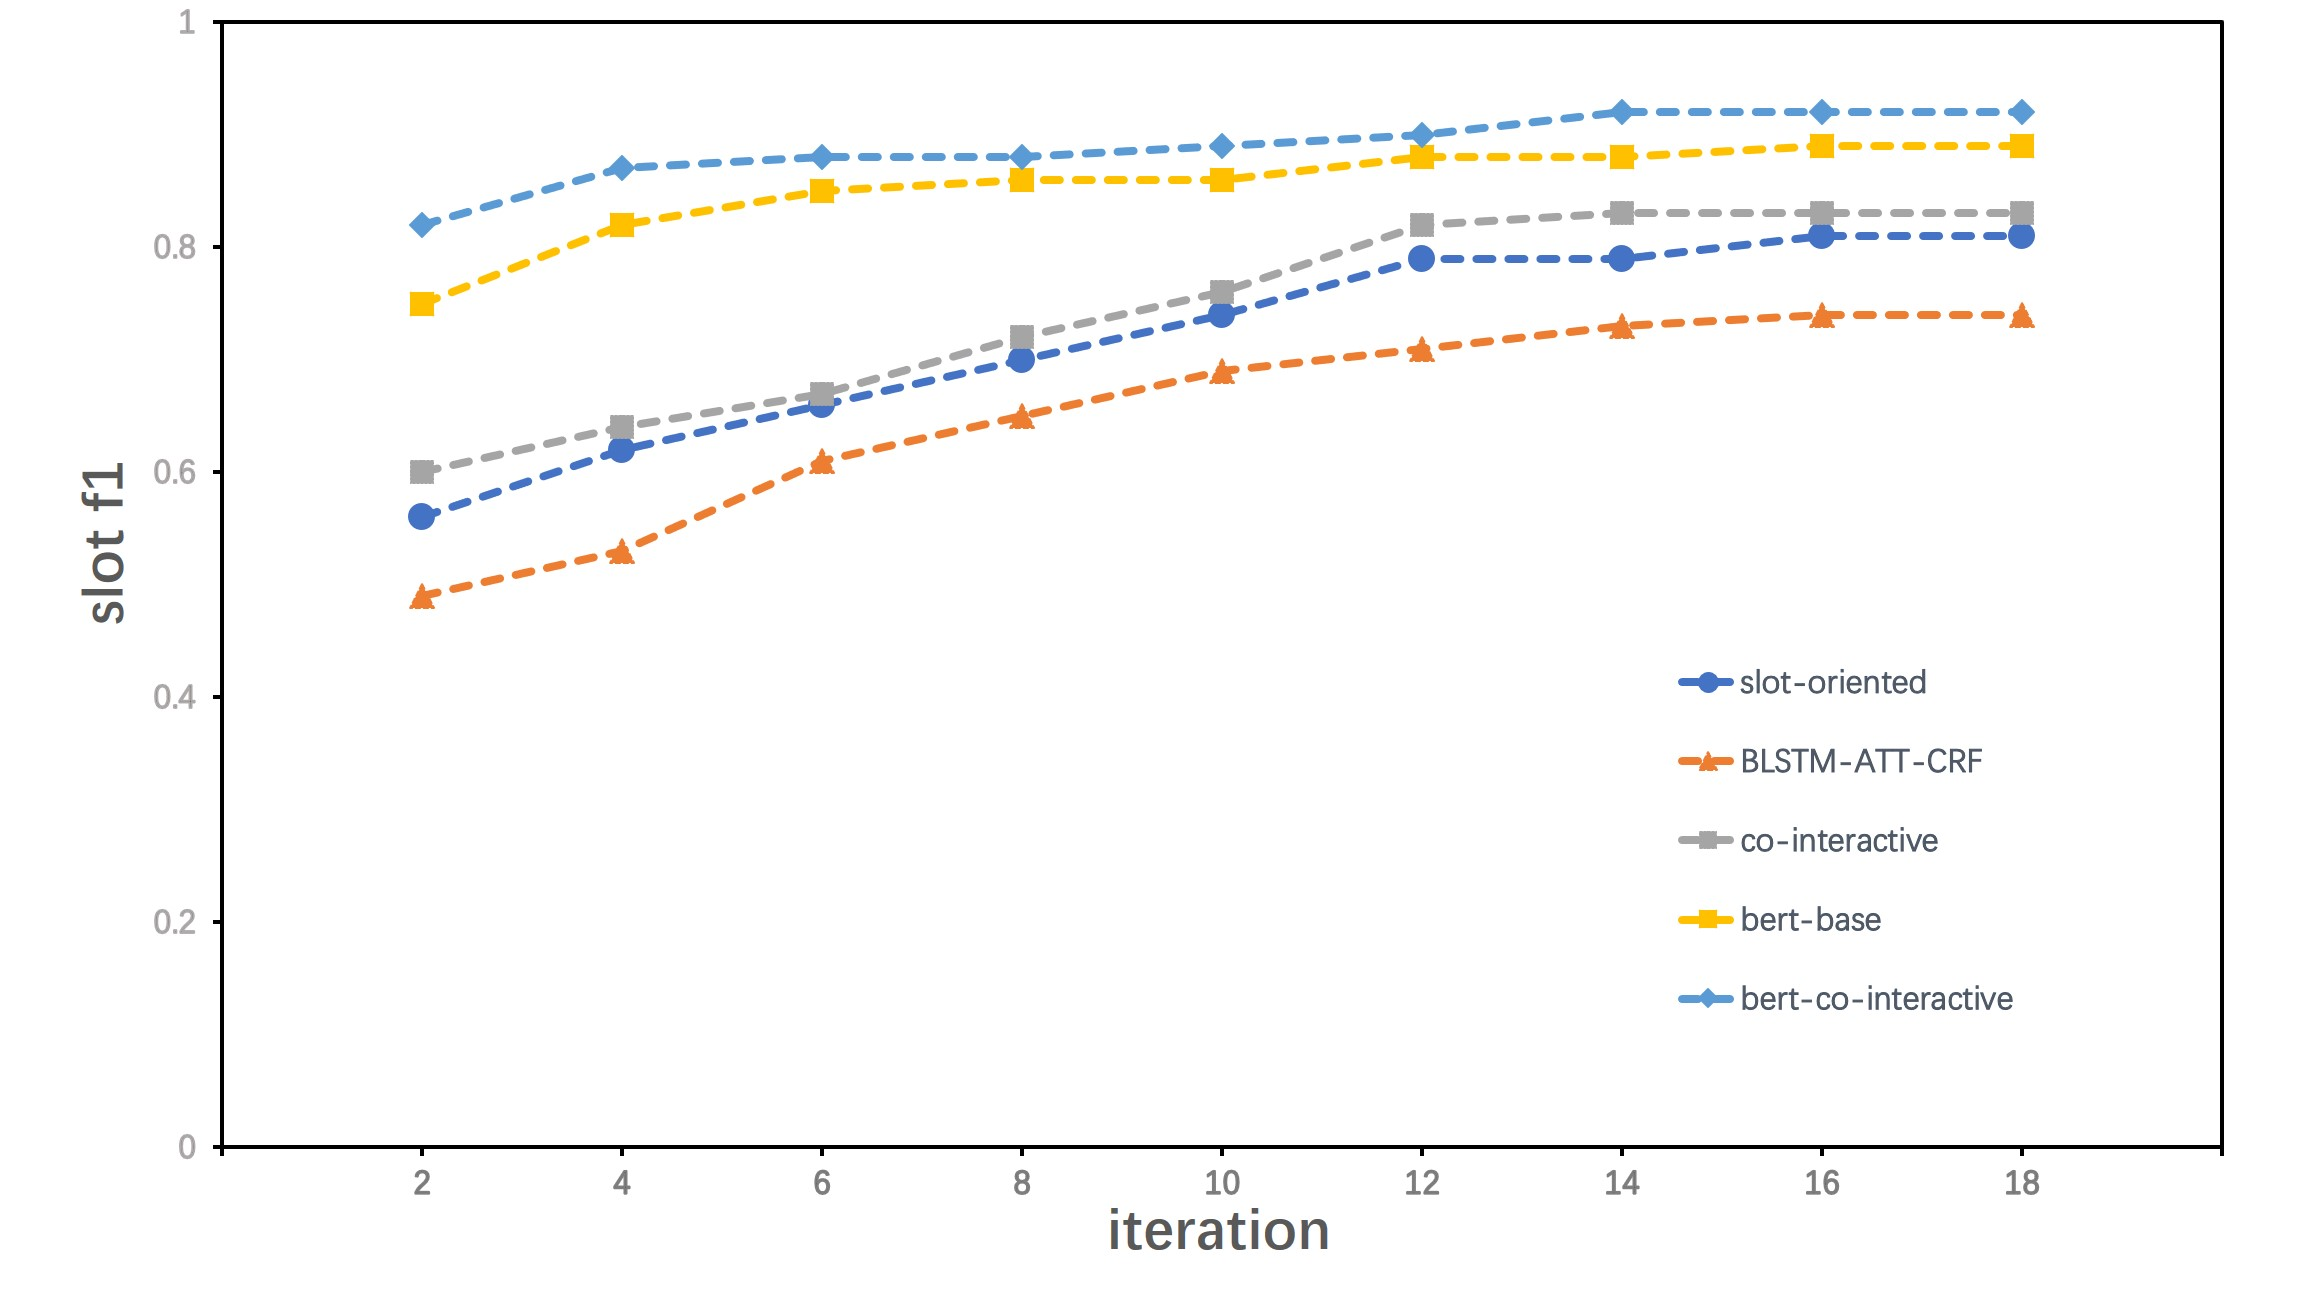
\includegraphics[width=8.6cm]{./images/slotF1.jpg}
  \label{fig:slotF1}
  }
  % \hspace{5pt}
  %  \hspace{+5mm}
  \subfloat[句子整体的accuracy曲线]{
  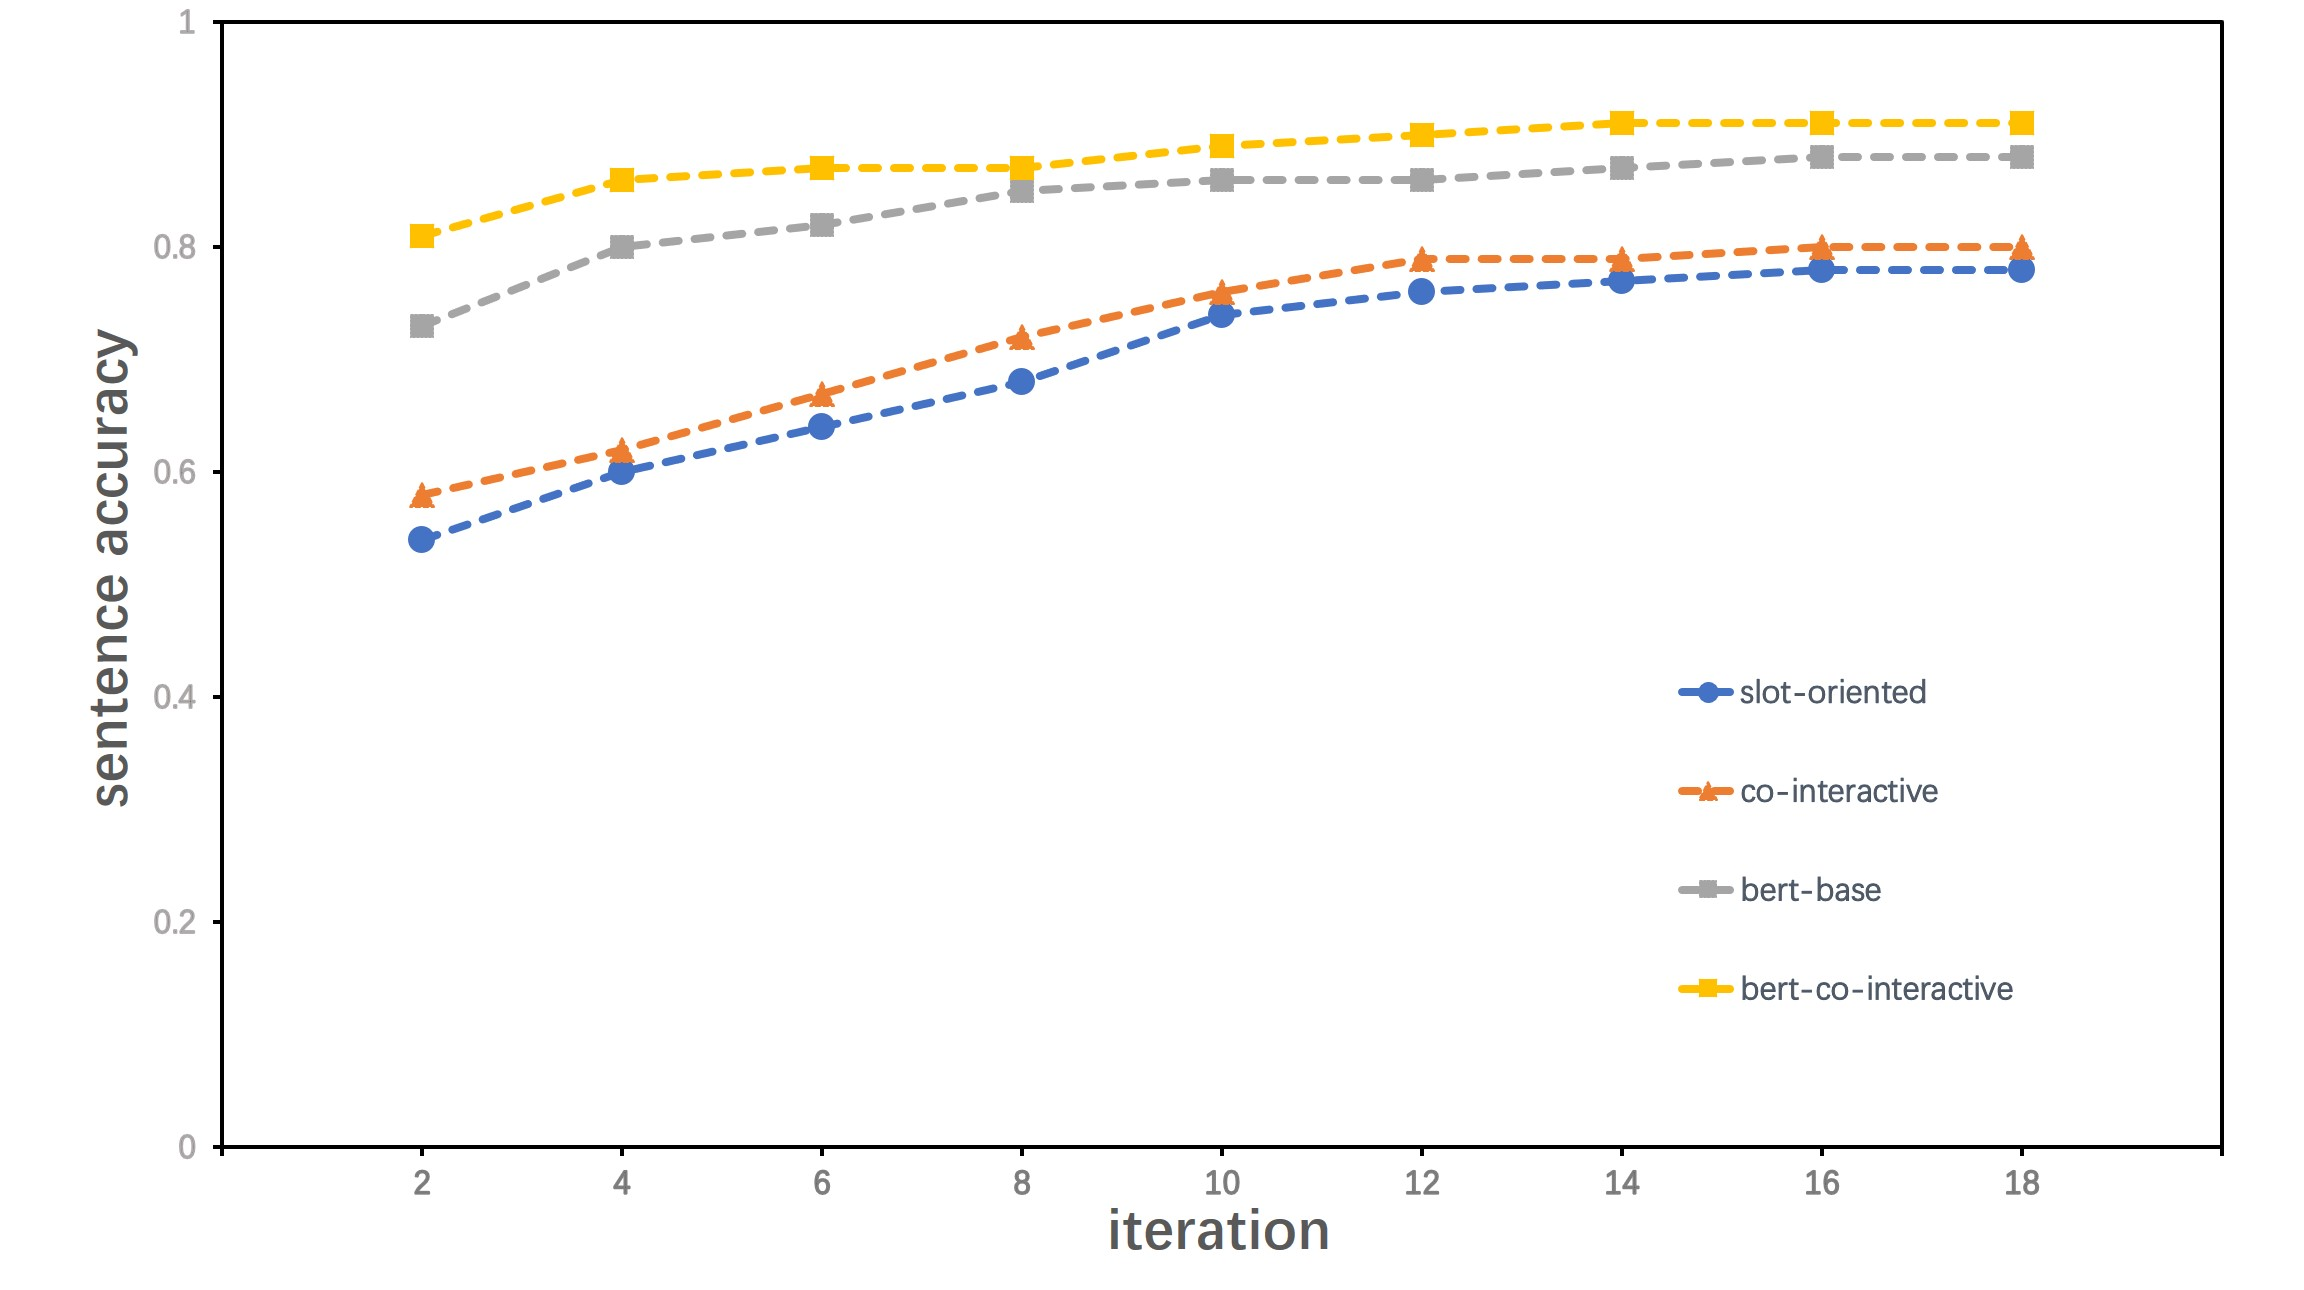
\includegraphics[width=8.6cm]{./images/sentenceAccuracy.jpg}
  \label{fig:sentenceAccuracy}
  }
  \caption{训练集上各模型指标值的变化}
  \label{fig:4}
  \end{figure}

  实验训练过程中模型的accuracy指标以及$F_1$指标变化如图\ref{fig:4}所示,从图\ref{fig:serviceAccuracy},\ref{fig:interfaceAccuracy}
  可以看到slot-oriented联合识别模型在服务分类和接口分类
  任务中表现不佳,不及ATT-CLSTM模型和Trans-CLSTM模型,原因是slot-oriented模型中信息流是从服务分类
  和接口分类传入语义槽填充,单向的流动并不能对信息源的任务带来增益。虽然如此,图\ref{fig:slotF1}显示,单向联合识别模型在语义槽填充任务上的表现
  优于BiLSTM-attention-CRF,原因在于得到了前两个任务的语义信息补充获得增益。

  预训练模型bert的引入为各项任务的性能带来了显著的提升,一方面,结合预训练的模型在经过较少轮的迭代就可以趋于收敛;
  另一方面,模型最终的指标得分也因为bert的引入而提高。这是由于bert的参数在预训练过程中使用了数据量庞大的语料,
  具有了对许多中文语句很好的理解和编码能力,同时本文的数据集中语料数量有限,导致其他模型不能很好的收敛,最终如图\ref{fig:sentenceAccuracy}显示
  结合预训练bert的模型在句子整体的准确率也是最优。

  \begin{table}[htb]
    \centering
    \caption{实验结果表}
    \label{tab:jieguo}
\begin{tabular}{l|cccc}
  \toprule
  \multicolumn{1}{c|}{\centering model}&Service Acc&Interface Acc&Slot $F_1$&Sentence Acc\\
   \hline
   ATT-CLSTM&84.37\%&-&-&-\\
   Trans-CLSTM&-&82.65\%&-&-\\
   BLSTM-ATT-CRF&-&-&74.19\%&-\\
   Slot-oriented&82.13\%&82.09\%&81.83\%&78.31\%\\
   Co-interactive&86.54\%&85.53\%&83.62\%&80.13\%\\
   BERT-base&93.72\%&91.26\%&88.01\%&87.63\%\\
   BERT-co-interactive&$\mathbf{95.18\%}$&$\mathbf{94.91}\%$&$\mathbf{92.23}\%$&$\mathbf{91.47}\%$\\
  \bottomrule
  \end{tabular}
\end{table}

本文所有模型的实验结果如表\ref{tab:jieguo}所示,以下是对结果数据的展开分析。
在多个任务中,对比结合预训练的模型和传统深度学习模型,“bert+”模式的结构对性能有很大的提升,这也证明了bert在语义理解任务中的作用和重要意义。
传统的深度学习方法不及“bert+”模式的原因在于训练的数据集有限,模型训练不充分,导致泛化能力较弱,而bert已在大规模语料训练中对下游任务有了初步的建模。

对于服务分类、接口分类和参数提取(语义槽填充)这三项强相关的任务,从其他任务中获得决策信息对当前任务的预测大有裨益,实验结果也验证了这一猜想,
slot-oriented联合识别模型由于获得了服务类别和接口类别信息,在参数提取(语义槽填充)任务上的$F_1$值相较于BiLSTM-attention-CRF有所提升,前两项任务表现
不佳是由于服务和接口的分类预测时并没有获得其他任务的决策信息增益,相反的,单向联合在前两项任务中设计的十分简单,
co-interactive联合识别模型则在三项任务中都有超过传统深度学习模型的表现。
\begin{figure}[htbp]
   \centering
  % \hspace{-7mm}
  \subfloat[第一层]{
  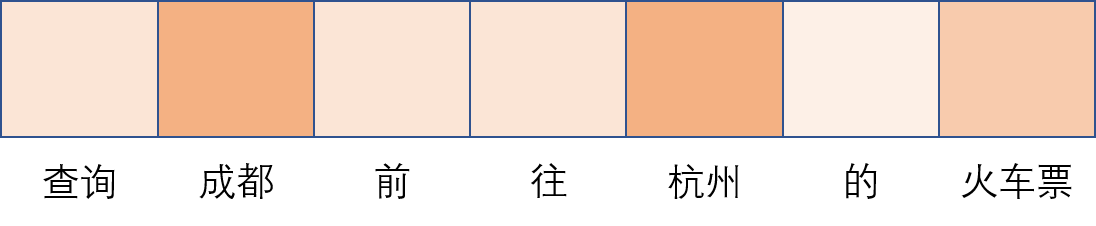
\includegraphics[width=8cm]{./images/first.png}
  \label{fig:777}
  }\\
  % \hspace{5pt}
    % \hspace{+5mm}
    \centering
  \subfloat[第二层]{
  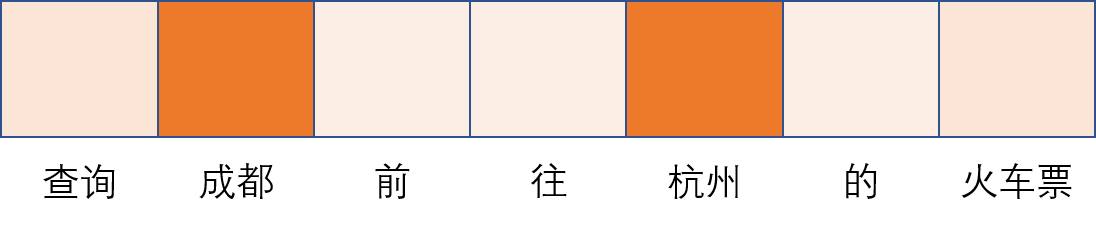
\includegraphics[width=8cm]{./images/second.png}
  \label{fig:77777}
  }
  \caption{协同交互层slot向量可视化}
  \label{fig:visual}
  \end{figure}
从bert-base和bert-co-interactive联合识别两组模型的对比中可以看出,相较于基础的softmax分类,在预训练模型上增加针对于语义理解的结构,模型效果会有所提升。
其中语义槽填充任务效果提升最为明显,原因是该任务相比于分类更为复杂,要求模型对语义理解的精度更高,因此模型之间在此任务之上表现的区分度很高。

对于测试集表现最优的bert-co-interactive联合识别模型,我们进行了进一步消融分析。消融分析直白的解释就是将模型视作pipeline,在模型整体性能较好的前提下,
我们希望分析出管道中结构A,B,C等对性能的影响,逐个剔除A,B,C做控制变量法的对比实验,探索模型中各模块对性能的影响和贡献,消融分析实验结果如表\ref{tab:xiaorongjieguo}所示。
首先bert预训练层的移除对实验结果影响巨大,各指标断崖式下跌,可见bert的引入对结果至关重要。
之后我们分别剔除了service attention层,interface attention层和slot attention层,将共享编码层的输出$\mathbf{H}$=[$h_{1}$,$h_{2}$,\dots,$h_{n}$]直接
输入到交互层,三次实验结果显示,分类的准确率以及语义槽$F_1$值均有所下降,结果表明对编码层向量做初步的attention处理增强语义理解,对于多个任务之间的协同交互有帮助。
然后我们修改了交互层的结构,由原来的信息多项交互共享转为单向的信息传递,三次实验分别是服务、接口信息流向语义槽填充任务((service,interface)-to-slot),
接口、语义槽填充信息流向服务分类任务((interface,slot)-to-service),服务、语义槽填充信息流向接口分类任务((service,slot)-to-interface),我们
只保留了信息的单向流通,实验结果显示,单向的信息流动相比于交互式的互相增强,会对准确率造成影响,均有所下降,这表明
对服务分类、接口分类和参数提取(语义槽填充)之间的交互建模可以以一种相互增强的方式来增强这三项任务。相反,如果仅考虑信息流的单个方向作用,而忽略另一个任务信息
的反哺能力,则不能带到更优的结果。
\begin{table}[htb]
  \centering
  \caption{消融分析}
  \label{tab:xiaorongjieguo}
\begin{tabular}{l|cccc}
  \toprule
  \multicolumn{1}{c|}{\centering model}&Service Acc&Interface Acc&Slot $F_1$&Sentence Acc\\
 \hline
 删除bert&86.54\%&85.53\%&83.62\%&80.13\%\\
 删除service attention层&94.55\%&94.52\%&92.01\%&91.03\%\\
 删除interface attention层&95.02\%&93.51\%&91.99\%&91.12\%\\
 删除slot attention层&94.98\%&94.47\%&91.13\%&90.27\%\\
 (service,interface)-to-slot&93.47\%&93.85\%&91.99\%&90.46\%\\
 (service,slot)-to-interface&93.52\%&93.77\%&91.08\%&90.31\%\\
 (interface,slot)-to-service&94.53\%&93.81\%&91.12\%&90.02\%\\
 bert-co-interactive&$\mathbf{95.18\%}$&$\mathbf{94.91}\%$&$\mathbf{92.23}\%$&$\mathbf{91.47}\%$\\
\bottomrule
\end{tabular}
\end{table}

对于bert-co-interactive联合识别模型,我们也探讨了协同交互模块的堆叠层数量对性能的影响,对比实验如图\ref{fig:layerCompare}所示。
可以看到,N的值从1增加到2时各指标均有所提升,说明使用一定深度的层次堆叠可以带来更好的性能。,
这是因为协同交互模块堆叠在一起形成层次结构,使任务之间能够进行多次交互,从而实现增量捕获交互信息来达到彼此丰富,
进而更好地为任务之间交互建模,并学习相互间的知识。 
但是当堆叠的层数超过三层时,模型性能会变差,
这其中的原因可能是随着整个网络的深入,出现梯度消失或过度拟合问题。
最终模型超参数N被定为2。

\begin{figure}[htbp]
  % \centering
  % \hspace{-7mm}
  \subfloat[服务Service分类的accuracy曲线]{
  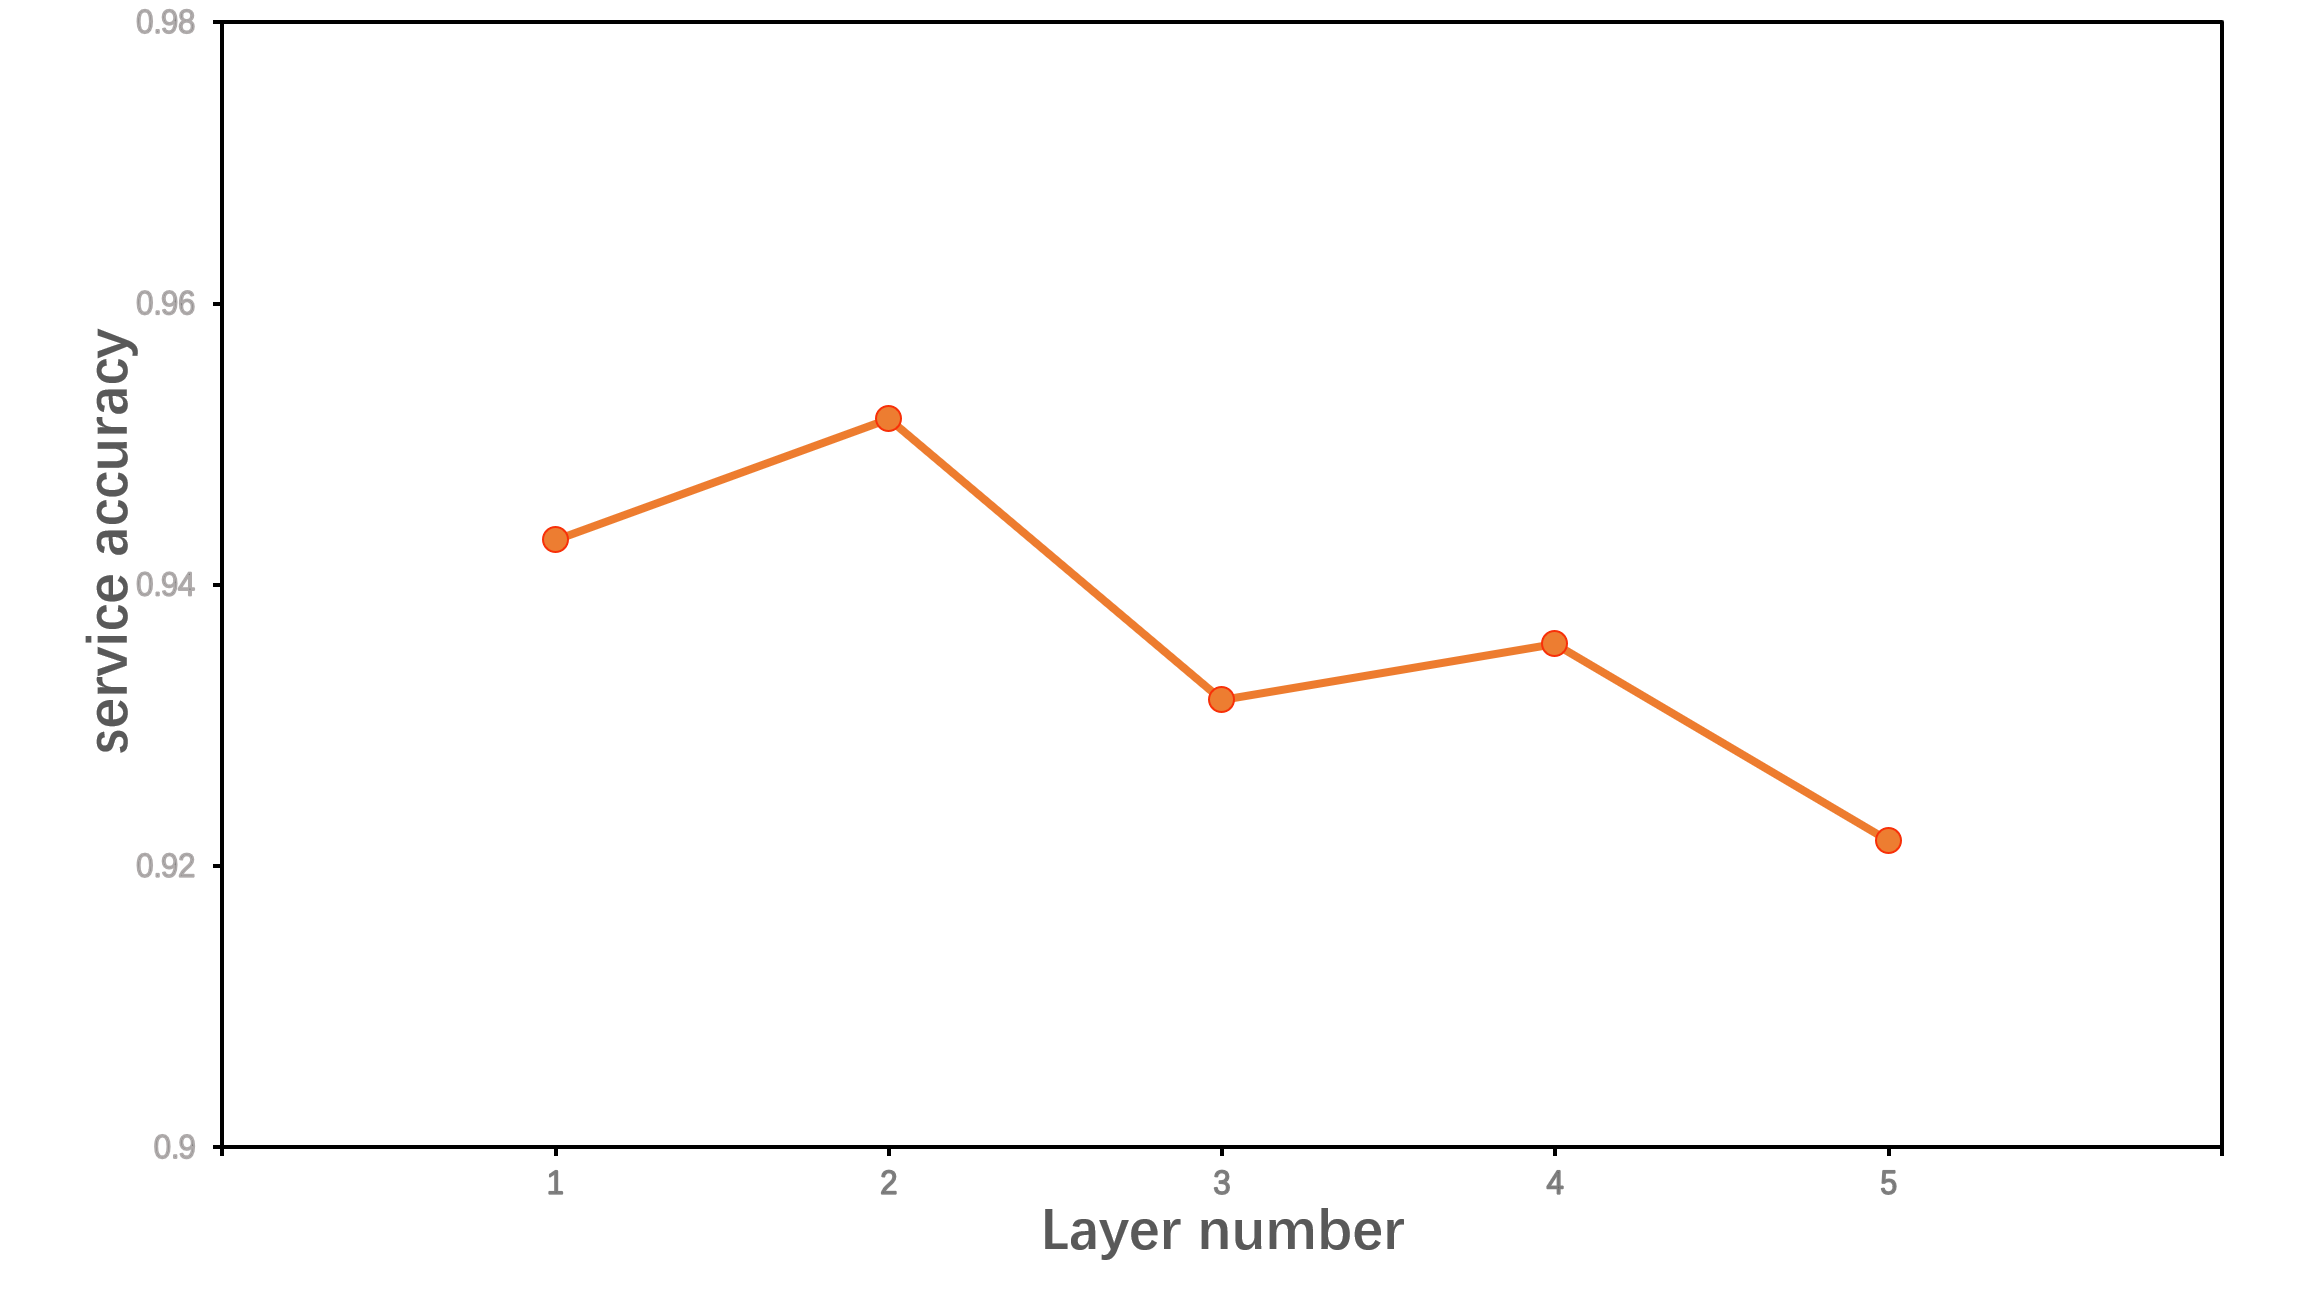
\includegraphics[width=8cm]{./images/layerService.png}
  \label{fig:serviceAccuracy2}
  }
  % \hspace{5pt}
    % \hspace{+5mm}
  \subfloat[接口Interface分类的accuracy曲线]{
  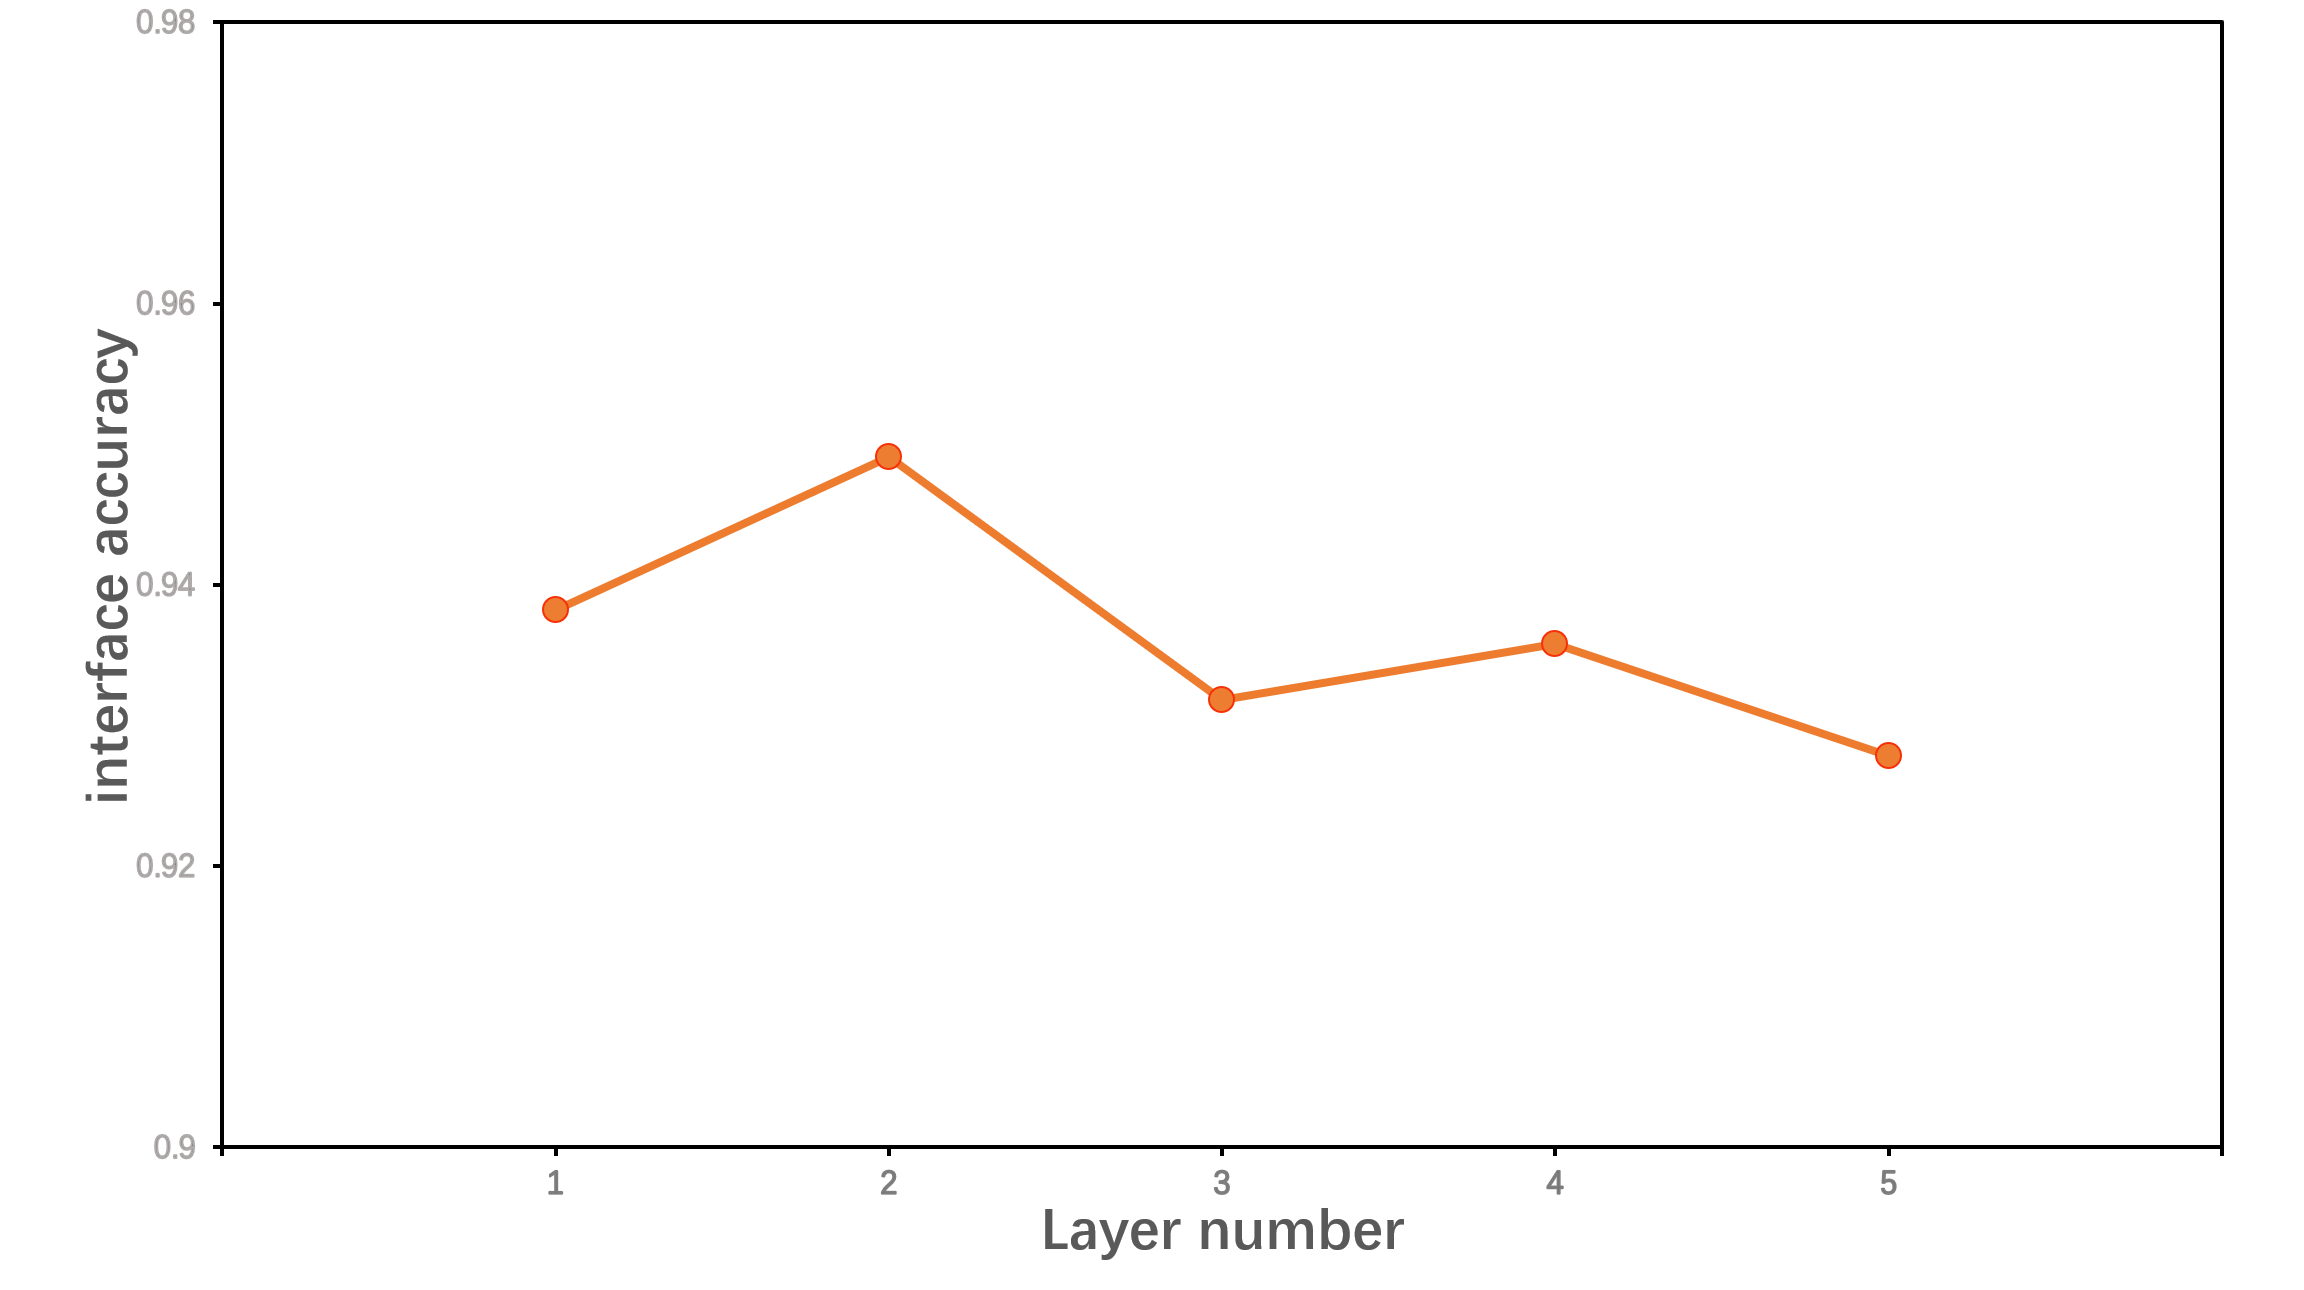
\includegraphics[width=8cm]{./images/layerInterface.png}
  \label{fig:interfaceAccuracy2}
  }\\
  % \hspace{5pt}
  %  \hspace{-7mm}
  \subfloat[语义槽填充的$F_1$曲线]{
  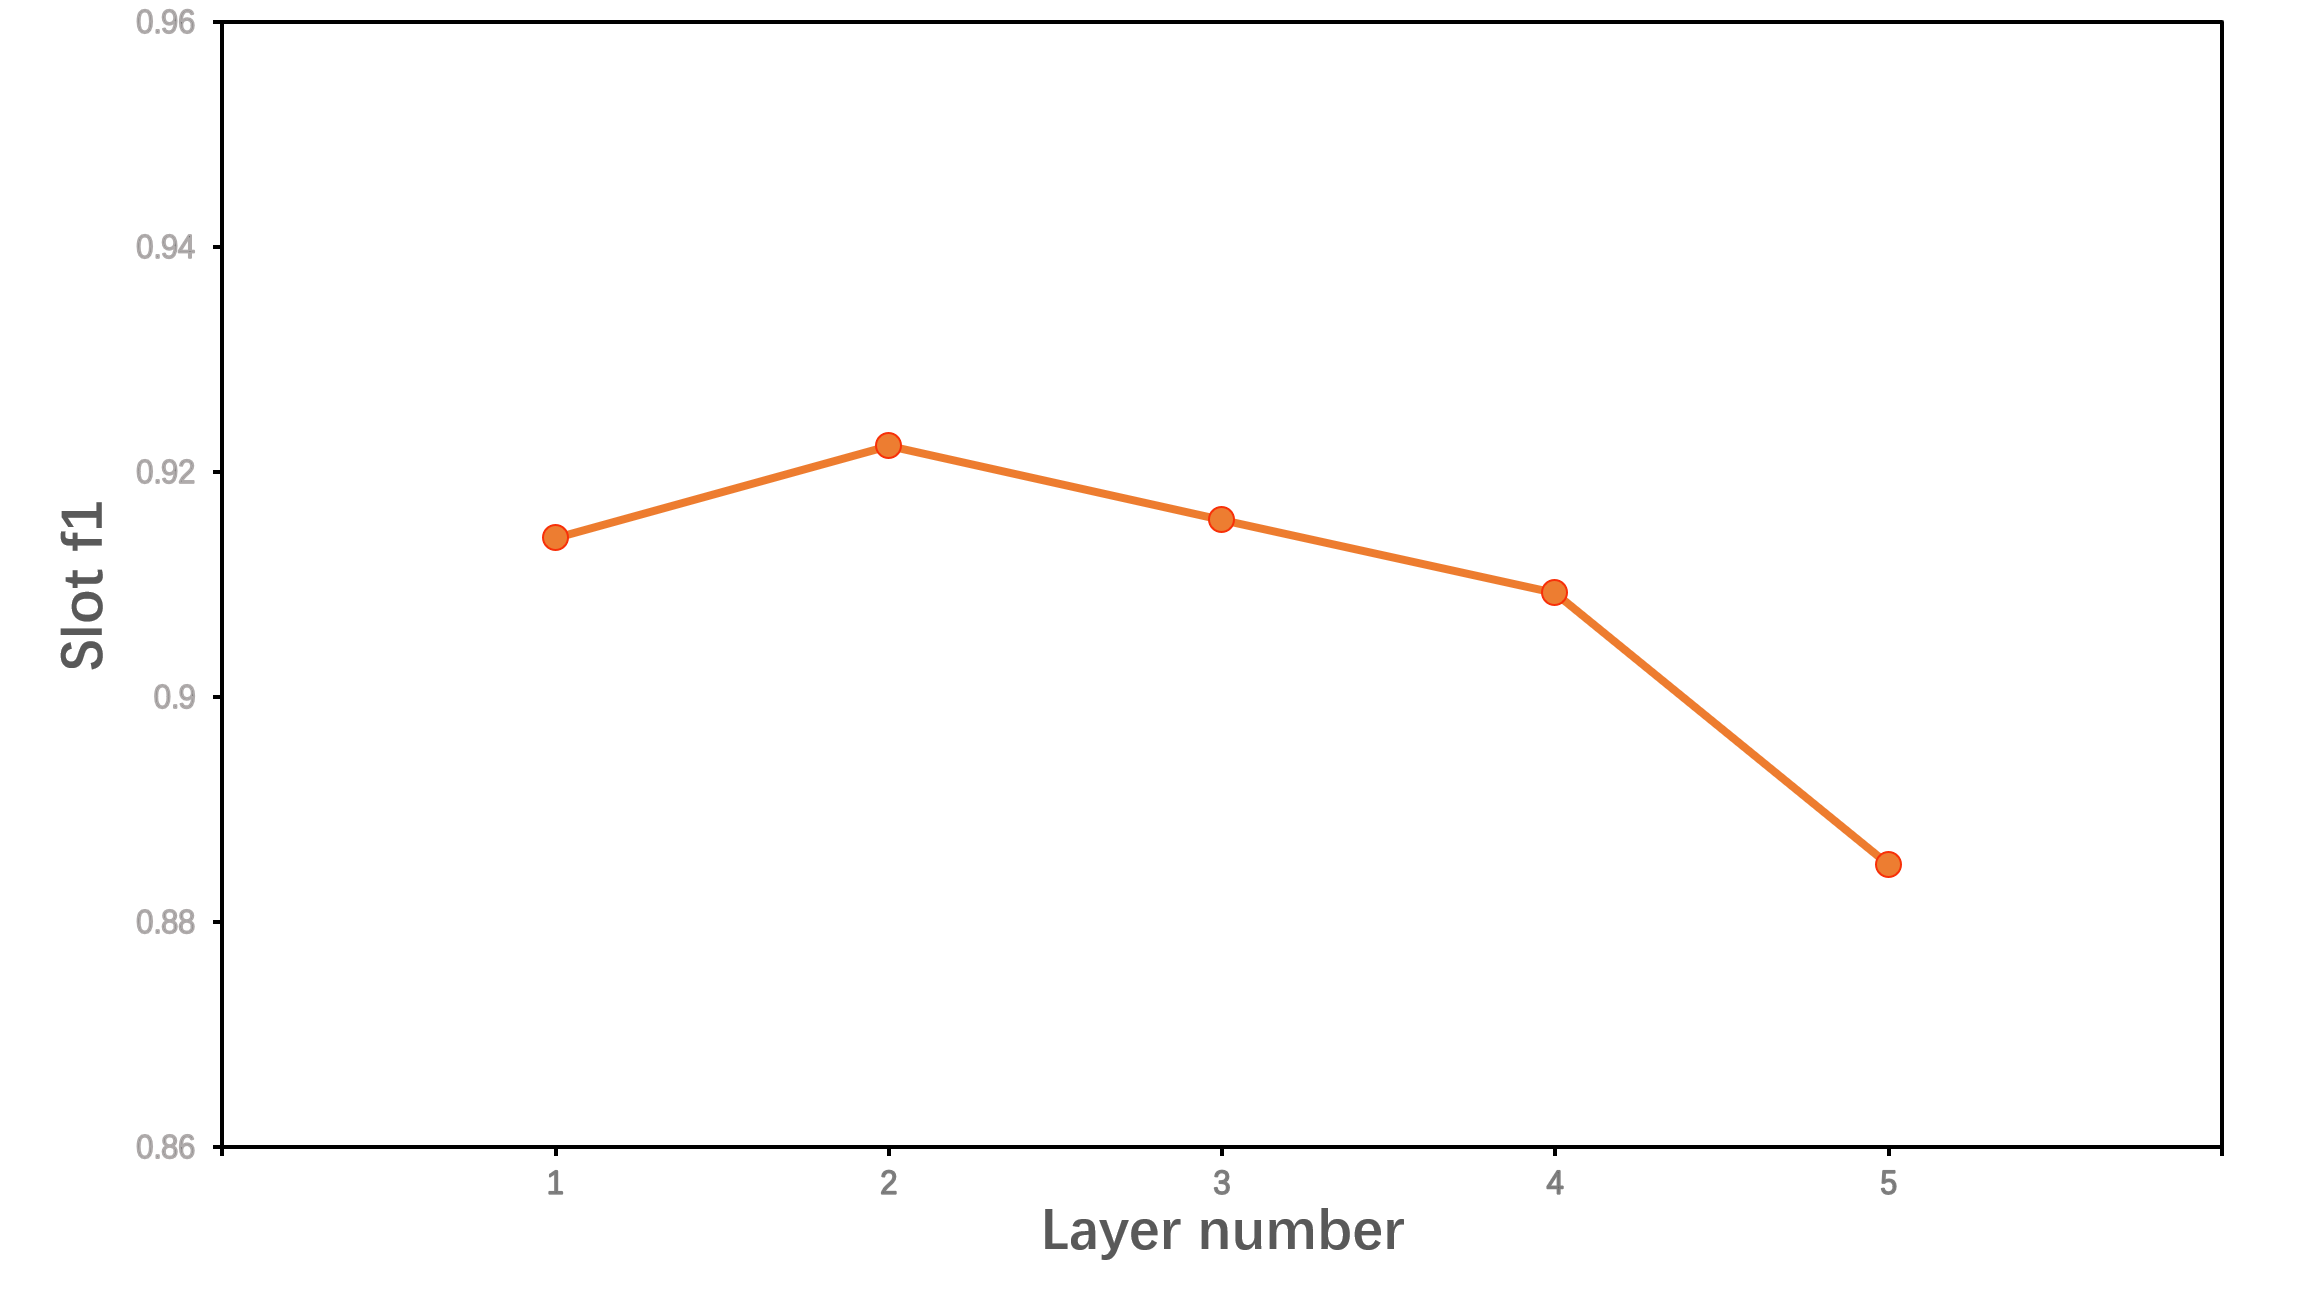
\includegraphics[width=8cm]{./images/layerSlot.png}
  \label{fig:slotF12}
  }
  % \hspace{5pt}
  %  \hspace{+5mm}
  \subfloat[句子整体的accuracy曲线]{
  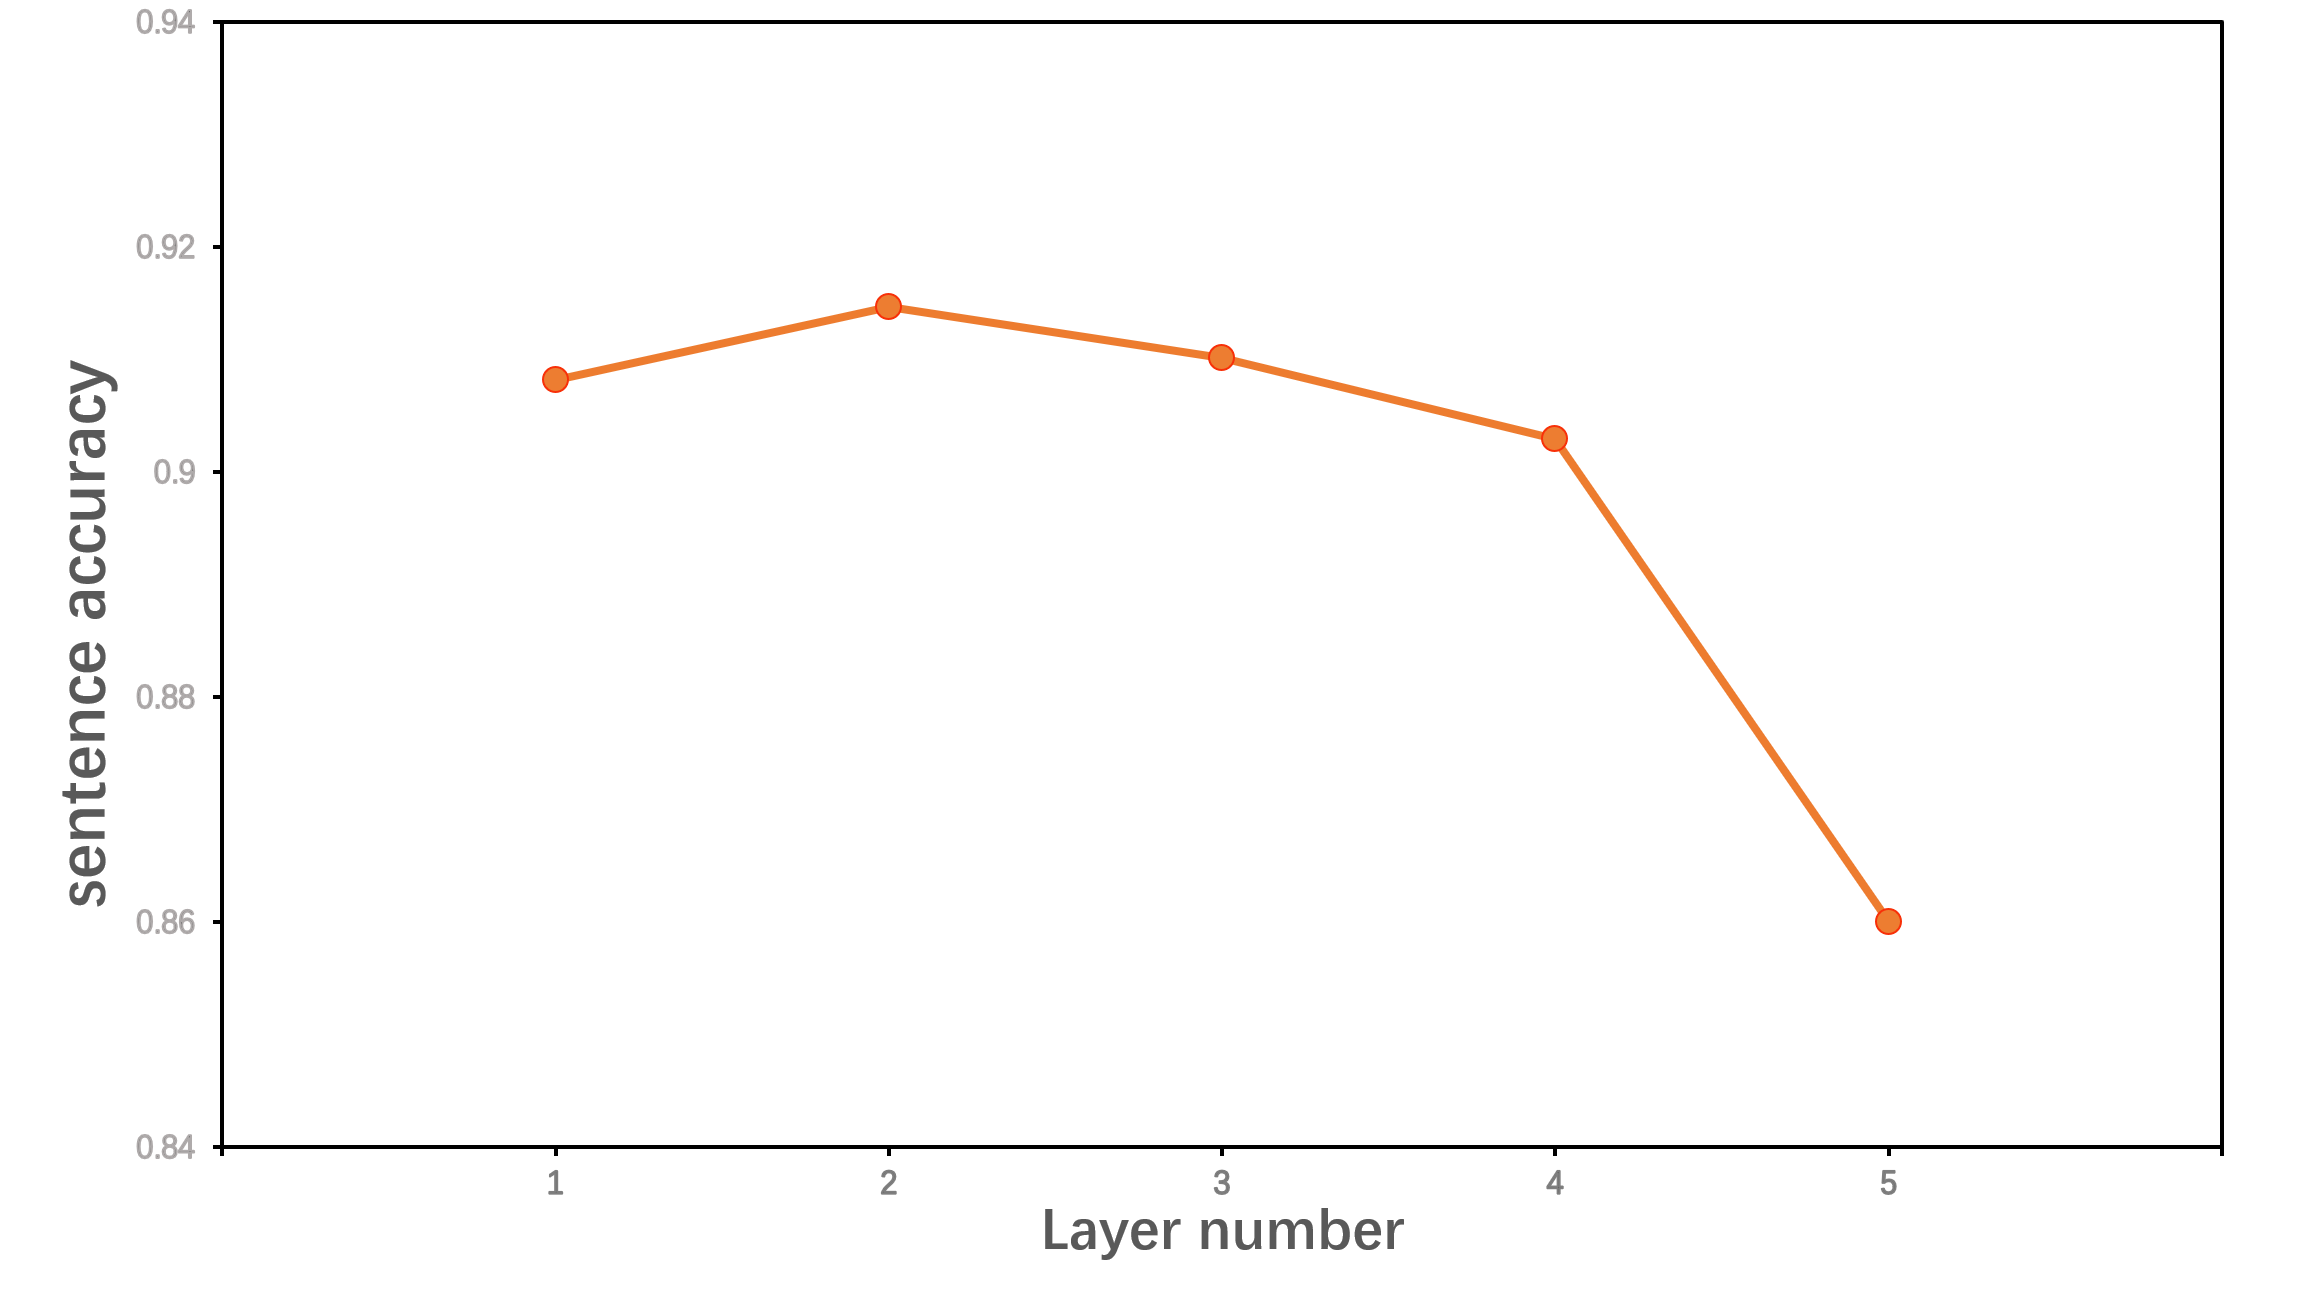
\includegraphics[width=8cm]{./images/layerSentence.png}
  \label{fig:sentenceAccuracy2}
  }
  \caption{bert-co-interactive不同堆叠层数模型性能比较}
  \label{fig:layerCompare}
  \end{figure}

  为了更好地了解模型学到了什么,让模型的设计更具可解释性,我们将co-interactive联合识别模型的协同交互层部分矩阵做了可视化处理\ref{fig:visual}。
  对于参数提取(语义槽填充)任务,在co-interactive联合识别模型的协同交互层中进行信息交互时,主要做了
  参数填充向量视为查询$Q_S$,服务分类向量视为键$K_D$以及值$K_D$,以获取可感知参数填充信息的服务分类向量表示信息并反馈给参数填充任务;
接口分类向量视为键$K_I$以及值$K_I$,以获取可感知参数填充信息的接口向量表示信息并反馈给参数填充任务。
  为此,我们将$Q_S$,$K_D$,$K_D$计算后的矩阵可视化,它表示了服务分类向量指导下各语义槽受到的注意力分布,
  从图中可以观察到:(1)我们的模型在服务类别向量“train”指导下正确地将注意权重完全集中在正确的语义槽(“成都”和“杭州”)上,
  这表明协同交互层任务间注意力机制可以指导模型学习。
  (2)使用更深的层(第二层)可以更好地帮助模型捕获相关的语义槽,与第一层相比,注意力着色更暗(表明得分高),
  这是因为协同交互模块堆叠在一起形成层次结构,使任务之间能够进行多次交互,从而实现增量捕获交互信息来达到彼此丰富。

  \section{本章小结}